\section{Past Work: Learning to Perceive, Reason, and Act through Tools with Multimodal RL}

\begin{frame}{\Large Starting with Visual Reasoning RL}
  \centering
  \vspace{-0.50cm}
  {\fontsize{11}{11}\selectfont
  I use visual reasoning RL as a first step toward improving the reasoning capability of multimodal agents under current observations.}

  \vspace{0.50cm}
  \begin{tikzpicture}[
    rootfade/.style={
      rounded corners=5pt,
      draw=AgentBlueDark!55,
      fill=AgentGray,
      very thick,
      minimum height=0.95cm,
      align=center,
      opacity=\SpotlightFadeOpacity,
      text opacity=\SpotlightFadeOpacity
    },
    activeouter/.style={
      rounded corners=5pt,
      draw=AgentBlueDark!75,
      fill=AgentGray,
      very thick,
      minimum width=4.15cm,
      minimum height=1.42cm,
      inner sep=0pt
    },
    fadeouter/.style={
      rounded corners=5pt,
      draw=AgentBlueDark!55,
      fill=AgentGray,
      very thick,
      minimum width=4.15cm,
      minimum height=1.42cm,
      inner sep=0pt,
      opacity=\SpotlightFadeOpacity
    },
    arrowfade/.style={-Latex,thick,draw=AgentBlueDark!80,opacity=\SpotlightFadeOpacity},
    arrowactive/.style={-Latex,thick,draw=AgentBlueDark!80},
    boundary/.style={thick,draw=AgentBlueDark!45,opacity=\SpotlightFadeOpacity}
  ]
    \node[rootfade,minimum width=1.8cm] (rl) at (-2.5,1.45) {\textbf{RL}};
    \node[rootfade,minimum width=3.7cm] (models) at (1.5,1.45) {\textbf{Multimodal Models \tiny(e.g. VLMs)}};
    \draw[arrowfade] (rl.east) -- (models.west);

    \node[activeouter] (reason) at (-5.0,-0.80) {};
    \begin{scope}
      \clip[rounded corners=5pt] (reason.south west) rectangle (reason.north east);
      \fill[AgentBlue] (reason.north west) rectangle ([yshift=-0.50cm]reason.north east);
    \end{scope}
    \node[rounded corners=5pt,draw=AgentBlueDark!75,very thick,minimum width=4.15cm,minimum height=1.42cm,inner sep=0pt]
      at (reason.center) {};
    \node[minimum width=4.10cm,minimum height=0.50cm,anchor=north,inner sep=0pt]
      at ([yshift=-0.03cm]reason.north) {\parbox{3.8cm}{\centering\fontsize{9}{9}\selectfont\bfseries Visual Reasoning}};
    \node[minimum width=4.10cm,minimum height=0.86cm,anchor=south,inner sep=0pt]
      at ([yshift=0.03cm]reason.south) {\parbox{3.75cm}{\centering\fontsize{8.2}{10}\selectfont Reshapes training dynamics\\and improves generalization}};

    \node[fadeouter] (unified) at (0,-0.80) {};
    \begin{scope}
      \clip[rounded corners=5pt] (unified.south west) rectangle (unified.north east);
      \fill[AgentBlue,opacity=\SpotlightFadeOpacity] (unified.north west) rectangle ([yshift=-0.50cm]unified.north east);
    \end{scope}
    \node[rounded corners=5pt,draw=AgentBlueDark!55,opacity=\SpotlightFadeOpacity,very thick,minimum width=4.15cm,minimum height=1.42cm,inner sep=0pt]
      at (unified.center) {};
    \node[minimum width=4.10cm,minimum height=0.50cm,anchor=north,inner sep=0pt,text opacity=\SpotlightFadeOpacity]
      at ([yshift=-0.03cm]unified.north) {\parbox{3.8cm}{\centering\fontsize{9}{9}\selectfont\bfseries Perception + Reasoning}};
    \node[minimum width=4.10cm,minimum height=0.86cm,anchor=south,inner sep=0pt,text opacity=\SpotlightFadeOpacity]
      at ([yshift=0.03cm]unified.south) {\parbox{3.75cm}{\centering\fontsize{8.2}{10}\selectfont Positive transfer under joint\\multimodal RL training}};

    \node[fadeouter] (tool) at (5.0,-0.80) {};
    \begin{scope}
      \clip[rounded corners=5pt] (tool.south west) rectangle (tool.north east);
      \fill[AgentBlue,opacity=\SpotlightFadeOpacity] (tool.north west) rectangle ([yshift=-0.50cm]tool.north east);
    \end{scope}
    \node[rounded corners=5pt,draw=AgentBlueDark!55,opacity=\SpotlightFadeOpacity,very thick,minimum width=4.15cm,minimum height=1.42cm,inner sep=0pt]
      at (tool.center) {};
    \node[minimum width=4.10cm,minimum height=0.50cm,anchor=north,inner sep=0pt,text opacity=\SpotlightFadeOpacity]
      at ([yshift=-0.03cm]tool.north) {\parbox{3.8cm}{\centering\fontsize{9}{9}\selectfont\bfseries Vision Tool-Use}};
    \node[minimum width=4.10cm,minimum height=0.86cm,anchor=south,inner sep=0pt,text opacity=\SpotlightFadeOpacity]
      at ([yshift=0.03cm]tool.south) {\parbox{3.75cm}{\centering\fontsize{8.2}{10}\selectfont Intrinsic learning dominates\\RL reduces tool-induced harm}};

    \draw[boundary] (rl.south west) to[out=235,in=75] (reason.north west);
    \draw[boundary] (models.south east) to[out=-45,in=105] (tool.north east);
    \draw[arrowfade] (reason.east) -- (unified.west);
    \draw[arrowfade] (unified.east) -- (tool.west);
  \end{tikzpicture}

  \vspace{0.85cm}
  {\fontsize{10.5}{12}\selectfont
  \textbf{First question:} how can we make claims about multimodal reasoning RL trustworthy?}
\end{frame}

\molochset{progressbar=foot}

\begin{frame}{\Large How Can We Make Claims About Multimodal Reasoning RL
Trustworthy?}
  \centering
  \vspace{0.10cm}
  {\fontsize{8.5}{11}\selectfont Early multimodal RL was hard to interpret from final tables and heterogeneous codebases. I built a transparent from-scratch VLM-RL framework and evaluated \underline{full learning trajectories} on visual reasoning tasks.}

  \vspace{0.30cm}
  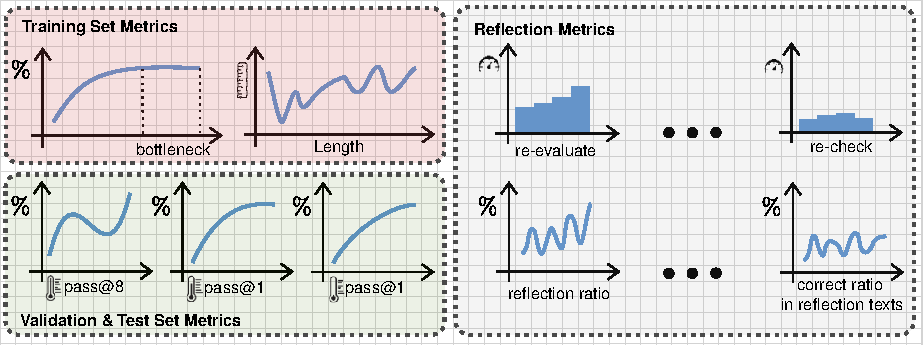
\includegraphics[width=0.75\linewidth]{figures/paper1/eval_scheme.pdf}

  \vspace{0.32cm}
  \begin{tikzpicture}[
    arrow/.style={-Latex,thick,draw=AgentBlueDark!75}
  ]
    \stacknode{traj}{(-3.6,0)}{Trajectory}{checkpoint-level dynamics}
    \stacknode{behavior}{(0,0)}{Behavior}{length and reflection metrics}
    \stacknode{gen}{(3.6,0)}{Generalization}{pass@\{1,k\} evaluation}
    \draw[arrow] (traj.east) -- (behavior.west);
    \draw[arrow] (behavior.east) -- (gen.west);
    \draw[
      decorate,
      decoration={brace,amplitude=4pt},
      thick,
      draw=AgentBlueDark!70
    ] ([xshift=0.33cm,yshift=0.41cm]gen.east)
      -- ([xshift=-0.15cm,yshift=-0.29cm]gen.east)
      node[midway,xshift=0.04cm,yshift=-0.08cm,anchor=west]
      {\scriptsize random seed};
  \end{tikzpicture}

  \vspace{-0.20cm}
  \begin{flushright}
    {\fontsize{5.5}{5}\selectfont \textcolor{darkgray}{[2025.01-2025.03]~~\textit{Rethinking RL Scaling for Vision Language Models: A Transparent, From-Scratch Framework and Comprehensive Evaluation Scheme}, Ma et al.}}
  \end{flushright}
\end{frame}

\molochset{progressbar=foot}

\begin{frame}{\Large What Does RL Change During Multimodal Reasoning Training?}
  \centering
  \vspace{0.05cm}
  {\fontsize{8.7}{10}\selectfont
  Trajectory-level evaluation reveals that RL changes how VLMs learn and respond, not only where final accuracy lands.}

  \vspace{0.15cm}
  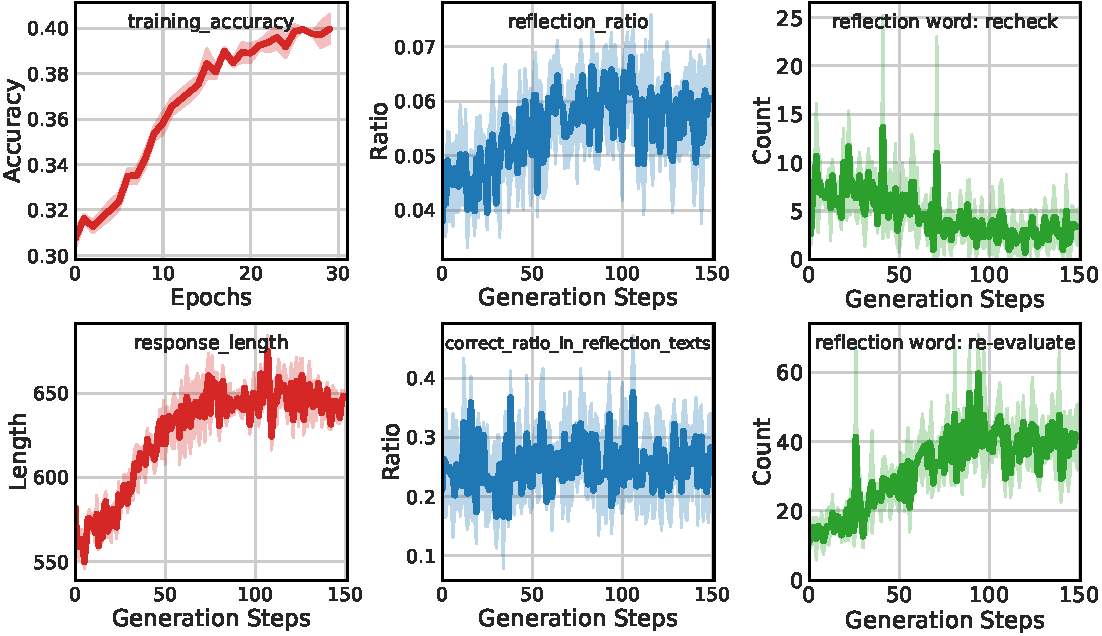
\includegraphics[width=0.62\linewidth]{figures/paper1/qwen2.5_mmmath_training_metrics.pdf}

  \vspace{0.15cm}
  \begin{tikzpicture}[
    metric/.style={
      rounded corners=4pt,
      draw=AgentBlueDark!45,
      fill=AgentGray,
      very thick,
      minimum width=2.65cm,
      minimum height=0.48cm,
      align=center,
      inner sep=2pt
    }
  ]
    \node[metric] at (-4.2,0) {\scriptsize Accuracy improves};
    \node[metric] at (-1.4,0) {\scriptsize Length shifts};
    \node[metric] at (1.4,0) {\scriptsize Reflection changes};
    \node[metric] at (4.2,0) {\scriptsize Seeds matter};
  \end{tikzpicture}

  \begin{flushright}
    {\fontsize{5.5}{5}\selectfont \textcolor{darkgray}{[2025.01-2025.03]~~\textit{Rethinking RL Scaling for Vision Language Models: A Transparent, From-Scratch Framework and Comprehensive Evaluation Scheme}, Ma et al.}}
  \end{flushright}
\end{frame}

\molochset{progressbar=foot}

\begin{frame}{\Large Do Multimodal RL Dynamics Look the Same Across Settings?}
  \centering
  {\fontsize{8}{10}\selectfont The same multimodal RL evaluation scheme reveals different dynamics across backbones and datasets.}

  \vspace{0.10cm}
  \begingroup
  \setlength{\tabcolsep}{3pt}
  \renewcommand{\arraystretch}{0.88}
  \begin{tabular}{@{}cc@{}}
    {\tiny Qwen2-VL-7B @ \textit{mm\_math5k}} &
    {\tiny Qwen2.5-VL-7B @ \textit{mm\_math5k}} \\
    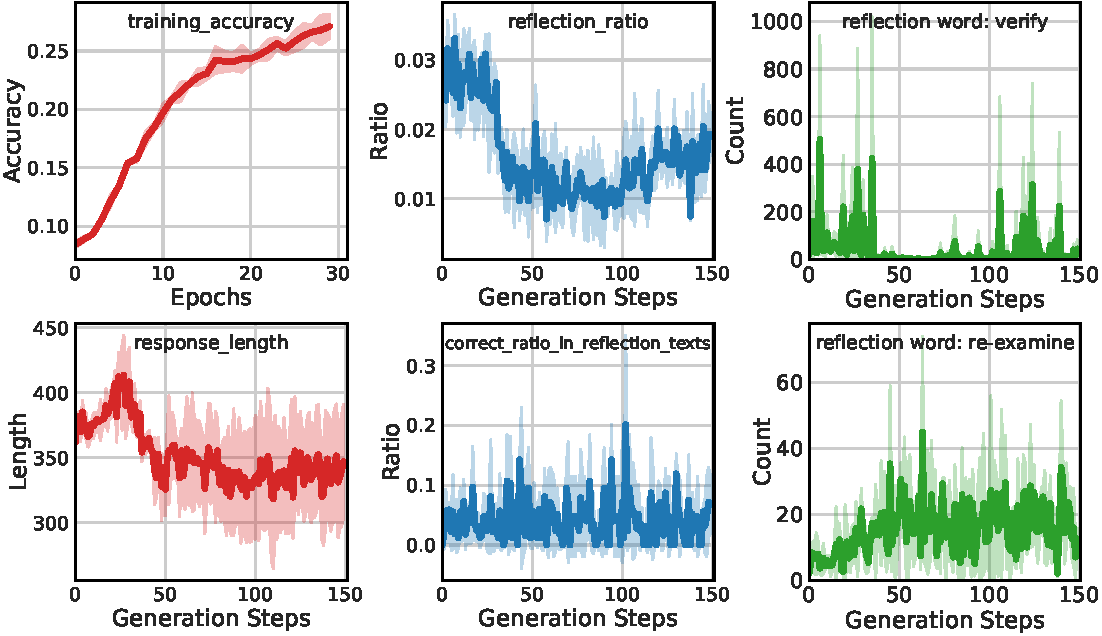
\includegraphics[width=0.36\linewidth]{figures/paper1/qwen2_mmmath_training_metrics.pdf} &
    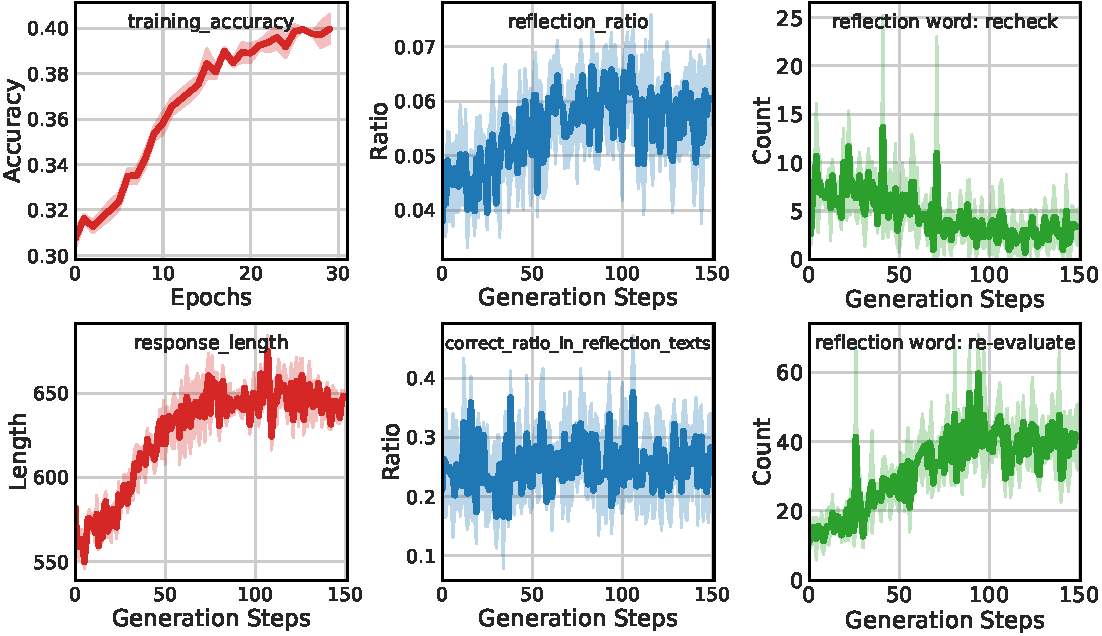
\includegraphics[width=0.36\linewidth]{figures/paper1/qwen2.5_mmmath_training_metrics.pdf} \\[-0.15em]
    {\tiny Qwen2-VL-7B @ \textit{geometry3k}} &
    {\tiny Qwen2.5-VL-7B @ \textit{geometry3k}} \\
    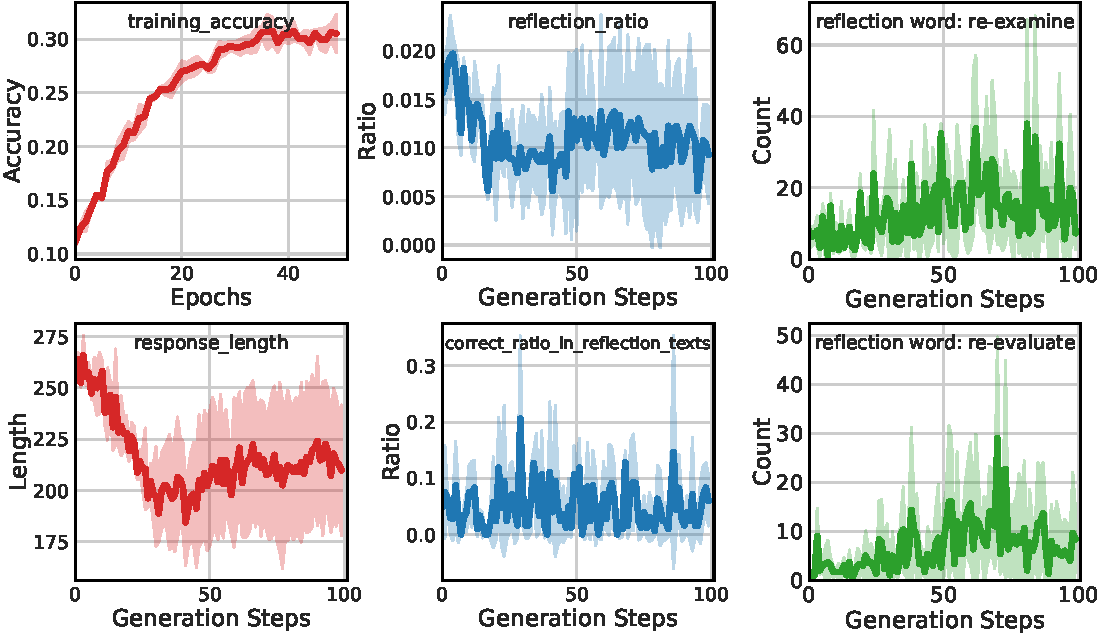
\includegraphics[width=0.36\linewidth]{figures/paper1/qwen2_geo3k_training_metrics.pdf} &
    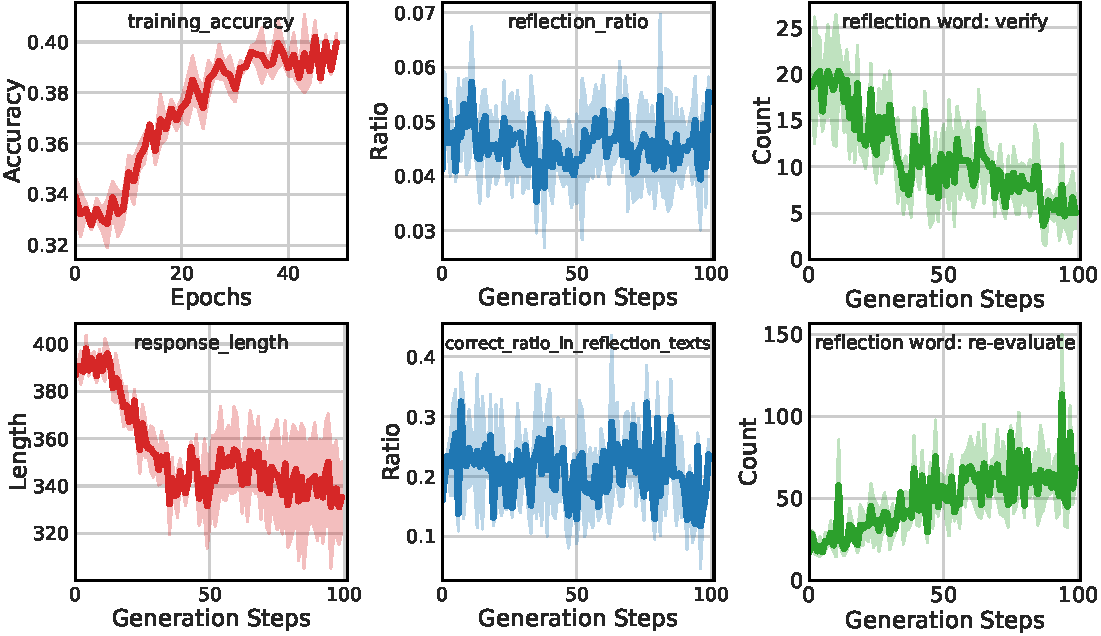
\includegraphics[width=0.36\linewidth]{figures/paper1/qwen2.5_geo3k_training_metrics.pdf}
  \end{tabular}
  \endgroup
  \begin{flushright}
    \vspace{-0.20cm}
    {\fontsize{5.5}{5}\selectfont \textcolor{darkgray}{[2025.01-2025.03]~~\textit{Rethinking RL Scaling for Vision Language Models: A Transparent, From-Scratch Framework and Comprehensive Evaluation Scheme}, Ma et al.}}
  \end{flushright}
\end{frame}

\molochset{progressbar=foot}

\begin{frame}{\Large Does Multimodal RL Change Generalization Beyond SFT?}
  \centering
  \vspace{0.10cm}
  {\fontsize{11}{10}\selectfont Compared with SFT on high-quality CoT solutions from textbooks, RL shows stronger validation/test generalization.}

  \vspace{0.18cm}
  \begingroup
  \setlength{\tabcolsep}{8pt}
  \renewcommand{\arraystretch}{0.90}
  \begin{tabular}{@{}cc@{}}
    {\scriptsize Qwen2-VL-7B @ \textit{mm\_math5k}} &
    {\scriptsize Qwen2.5-VL-7B @ \textit{mm\_math5k}} \\
    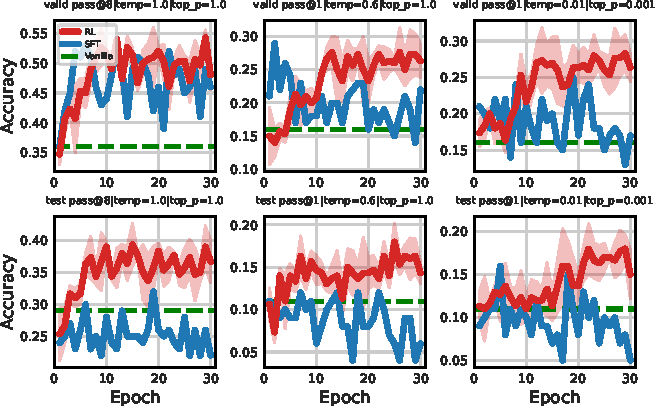
\includegraphics[width=0.49\linewidth]{figures/paper1/qwen2_rl_sft.pdf} &
    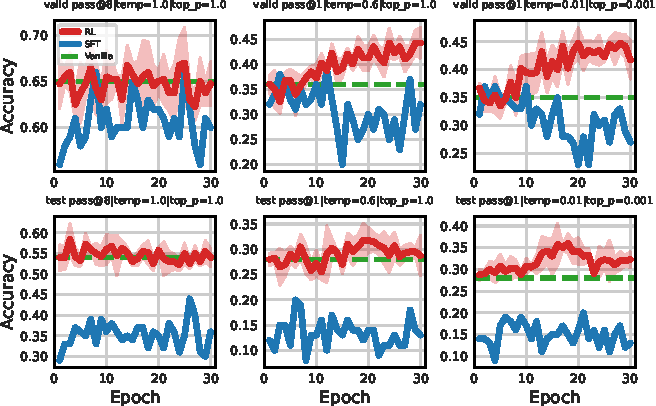
\includegraphics[width=0.49\linewidth]{figures/paper1/qwen2_5_rl_sft.pdf}
  \end{tabular}
  \endgroup

  \vspace{0.12cm}
  \begin{tikzpicture}
    \node[
      rounded corners=4pt,
      draw=AgentBlueDark!45,
      fill=AgentGray,
      very thick,
      inner xsep=9pt,
      inner ysep=5pt,
      align=center
    ] {\scriptsize RL improves generalization where SFT can overfit to supervised reasoning traces.};
  \end{tikzpicture}

  \begin{flushright}
    \vspace{0.05cm}
    {\fontsize{5.5}{5}\selectfont \textcolor{darkgray}{[2025.01-2025.03]~~\textit{Rethinking RL Scaling for Vision Language Models: A Transparent, From-Scratch Framework and Comprehensive Evaluation Scheme}, Ma et al.}}
  \end{flushright}
\end{frame}

\molochset{progressbar=foot}

\begin{frame}{\Large From Visual Reasoning to Perception + Reasoning}
  \centering
  \vspace{-0.40cm}
  {\fontsize{11}{11}\selectfont
  Reasoning decides how to think; perception determines whether the model is thinking about the right visual evidence.}

  \vspace{0.70cm}
  \begin{tikzpicture}[
    rootfade/.style={
      rounded corners=5pt,
      draw=AgentBlueDark!55,
      fill=AgentGray,
      very thick,
      minimum height=0.95cm,
      align=center,
      opacity=\SpotlightFadeOpacity,
      text opacity=\SpotlightFadeOpacity
    },
    activeouter/.style={
      rounded corners=5pt,
      draw=AgentBlueDark!75,
      fill=AgentGray,
      very thick,
      minimum width=4.15cm,
      minimum height=1.42cm,
      inner sep=0pt
    },
    fadeouter/.style={
      rounded corners=5pt,
      draw=AgentBlueDark!55,
      fill=AgentGray,
      very thick,
      minimum width=4.15cm,
      minimum height=1.42cm,
      inner sep=0pt,
      opacity=\SpotlightFadeOpacity
    },
    arrowfade/.style={-Latex,thick,draw=AgentBlueDark!80,opacity=\SpotlightFadeOpacity},
    arrowactive/.style={-Latex,thick,draw=AgentBlueDark!80},
    boundary/.style={thick,draw=AgentBlueDark!45,opacity=\SpotlightFadeOpacity}
  ]
    \node[rootfade,minimum width=1.8cm] (rl) at (-2.5,1.45) {\textbf{RL}};
    \node[rootfade,minimum width=3.7cm] (models) at (1.5,1.45) {\textbf{Multimodal Models \tiny(e.g. VLMs)}};
    \draw[arrowfade] (rl.east) -- (models.west);

    \node[fadeouter] (reason) at (-5.0,-0.80) {};
    \begin{scope}
      \clip[rounded corners=5pt] (reason.south west) rectangle (reason.north east);
      \fill[AgentBlue,opacity=\SpotlightFadeOpacity] (reason.north west) rectangle ([yshift=-0.50cm]reason.north east);
    \end{scope}
    \node[rounded corners=5pt,draw=AgentBlueDark!55,opacity=\SpotlightFadeOpacity,very thick,minimum width=4.15cm,minimum height=1.42cm,inner sep=0pt]
      at (reason.center) {};
    \node[minimum width=4.10cm,minimum height=0.50cm,anchor=north,inner sep=0pt,text opacity=\SpotlightFadeOpacity]
      at ([yshift=-0.03cm]reason.north) {\parbox{3.8cm}{\centering\fontsize{9}{9}\selectfont\bfseries Visual Reasoning}};
    \node[minimum width=4.10cm,minimum height=0.86cm,anchor=south,inner sep=0pt,text opacity=\SpotlightFadeOpacity]
      at ([yshift=0.03cm]reason.south) {\parbox{3.75cm}{\centering\fontsize{8.2}{10}\selectfont Reshapes training dynamics\\and improves generalization}};

    \node[activeouter] (unified) at (0,-0.80) {};
    \begin{scope}
      \clip[rounded corners=5pt] (unified.south west) rectangle (unified.north east);
      \fill[AgentBlue] (unified.north west) rectangle ([yshift=-0.50cm]unified.north east);
    \end{scope}
    \node[rounded corners=5pt,draw=AgentBlueDark!75,very thick,minimum width=4.15cm,minimum height=1.42cm,inner sep=0pt]
      at (unified.center) {};
    \node[minimum width=4.10cm,minimum height=0.50cm,anchor=north,inner sep=0pt]
      at ([yshift=-0.03cm]unified.north) {\parbox{3.8cm}{\centering\fontsize{9}{9}\selectfont\bfseries Perception + Reasoning}};
    \node[minimum width=4.10cm,minimum height=0.86cm,anchor=south,inner sep=0pt]
      at ([yshift=0.03cm]unified.south) {\parbox{3.75cm}{\centering\fontsize{8.2}{10}\selectfont Positive transfer under joint\\multimodal RL training}};

    \node[fadeouter] (tool) at (5.0,-0.80) {};
    \begin{scope}
      \clip[rounded corners=5pt] (tool.south west) rectangle (tool.north east);
      \fill[AgentBlue,opacity=\SpotlightFadeOpacity] (tool.north west) rectangle ([yshift=-0.50cm]tool.north east);
    \end{scope}
    \node[rounded corners=5pt,draw=AgentBlueDark!55,opacity=\SpotlightFadeOpacity,very thick,minimum width=4.15cm,minimum height=1.42cm,inner sep=0pt]
      at (tool.center) {};
    \node[minimum width=4.10cm,minimum height=0.50cm,anchor=north,inner sep=0pt,text opacity=\SpotlightFadeOpacity]
      at ([yshift=-0.03cm]tool.north) {\parbox{3.8cm}{\centering\fontsize{9}{9}\selectfont\bfseries Vision Tool-Use}};
    \node[minimum width=4.10cm,minimum height=0.86cm,anchor=south,inner sep=0pt,text opacity=\SpotlightFadeOpacity]
      at ([yshift=0.03cm]tool.south) {\parbox{3.75cm}{\centering\fontsize{8.2}{10}\selectfont Intrinsic learning dominates\\RL reduces tool-induced harm}};

    \draw[boundary] (rl.south west) to[out=235,in=75] (reason.north west);
    \draw[boundary] (models.south east) to[out=-45,in=105] (tool.north east);
    \draw[arrowactive] (reason.east) -- (unified.west);
    \draw[arrowfade] (unified.east) -- (tool.west);
  \end{tikzpicture}

  \vspace{0.55cm}
  {\fontsize{10.5}{12}\selectfont
  \textbf{Next question:} can multimodal RL improve both within one training pipeline?}
\end{frame}

\molochset{progressbar=foot}

\begin{frame}{\Large Can Multimodal RL Jointly Shape Perception and Reasoning?}
  \centering
  \vspace{0.24cm}
  {\fontsize{11}{10}\selectfont Under matched budgets, unified RL matches or outperforms specialist mixtures across both reasoning and perception.}

  \vspace{0.14cm}
  {
  \noindent
  \begin{minipage}[t]{0.30\textwidth}
    \vspace{0pt}
    \centering
    {\scriptsize MEGA-Bench task composition}\\[-0.15em]
    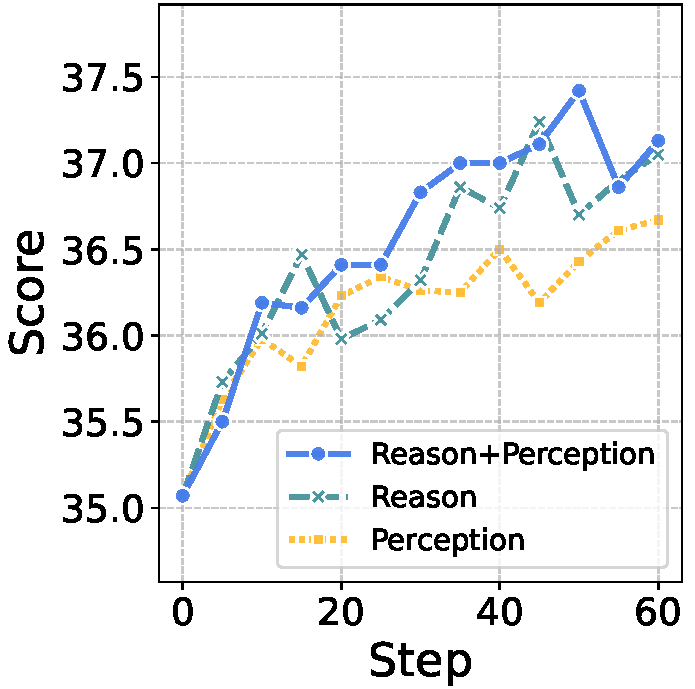
\includegraphics[width=0.98\linewidth]{figures/paper2/fair_budget_evidence_megabench.pdf}
  \end{minipage}
  \hfill
  \begin{minipage}[t]{0.68\textwidth}
\vspace{0pt}
\centering
\scriptsize
\setlength{\tabcolsep}{4pt}
\resizebox{\linewidth}{!}{%
\begin{tabular}{lccccc}
\toprule
\multicolumn{6}{c}{Reasoning Benchmarks} \\
\midrule
Mixture & MMMU & MathVista & MathVision & MME-R & CharXiv (RQ) \\
\midrule
Unified & \underline{56.56} & \underline{71.40} & \underline{30.51} & \textbf{28.20} & \textbf{44.50} \\
Reason-only & 54.89 & \textbf{71.70} & \textbf{31.24} & \underline{28.03} & \underline{44.00} \\
Perception-only & \textbf{56.67} & 68.20 & 29.59 & 26.26 & 41.00 \\
\bottomrule
\end{tabular}
}

\vspace{4pt}

\resizebox{\linewidth}{!}{%
\begin{tabular}{lccccc}
\toprule
\multicolumn{6}{c}{Perception Benchmarks} \\
\midrule
Mixture & HrBench4K & VStar & COCO (S$\mid$M) & OCRBenchV2 & ScreenSpot-Pro \\
\midrule
Unified & \underline{73.75} & \textbf{82.20} & \underline{80.69} $\mid$ \textbf{38.62} & \textbf{55.87} & \underline{23.91} \\
Reason-only & 73.25 & 78.53 & 78.36 $\mid$ 33.87 & \underline{55.77} & \textbf{23.97} \\
Perception-only & \textbf{76.00} & \underline{80.10} & \textbf{80.78} $\mid$ \underline{37.37} & 55.33 & 23.78 \\
\bottomrule
\end{tabular}
}
\end{minipage}


  \vspace{0.12cm}
  \tinytag{Reasoning: math / science / chart / puzzle}\hspace{0.25cm}
  \tinytag{Perception: detection / grounding / OCR / counting}\\[0.25em]
  \tinytag{47.7K verifiable samples}\hspace{0.25cm}
  \tinytag{Qwen2.5-VL 7B / 32B-0321/0326}}

  \vfill
  \begin{flushright}
    {\fontsize{5.5}{5}\selectfont \textcolor{darkgray}{[2025.04-2025.06]~~\textit{One RL to See Them All: Visual Triple Unified Reinforcement Learning}, Ma et al.}}
  \end{flushright}
\end{frame}

\molochset{progressbar=foot}

\begin{frame}{\Large How Can Unified Multimodal RL Handle Heterogeneous Tasks?}
  \vspace{0.00cm}
  \begin{columns}[T,onlytextwidth]
    \begin{column}{0.60\textwidth}
      \centering
      \vspace{0.40cm}
      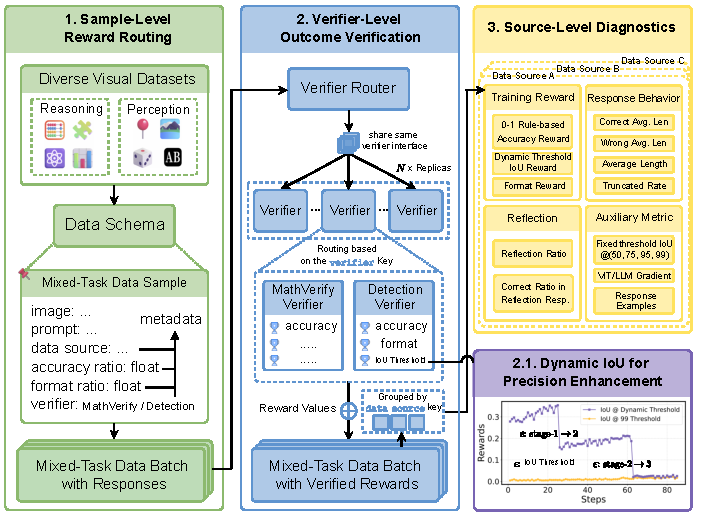
\includegraphics[width=0.98\linewidth]{figures/paper2/vtriune_framework.pdf}
    \end{column}
    \begin{column}{0.39\textwidth}
      \vspace{0.62cm}
      {\fontsize{9.2}{11}\selectfont
      We make heterogeneous multimodal tasks trainable in one RL loop.}

      \vspace{0.28cm}
      \begin{tikzpicture}[
        method/.style={
          rounded corners=4pt,
          draw=AgentBlueDark!45,
          fill=AgentGray,
          very thick,
          minimum width=4.75cm,
          minimum height=0.68cm,
          align=center,
          inner sep=2pt
        },
        arrow/.style={-Latex,semithick,draw=AgentBlueDark!55}
      ]
        \node[method] (routing) at (0,0) {\parbox{4.45cm}{\centering\small\textbf{Reward routing}\\[0.25em]\scriptsize handles sample-level heterogeneity}};
        \node[method] (verify) at (0,-1.85) {\parbox{4.45cm}{\centering\small\textbf{Outcome verification}\\[0.25em]\scriptsize handles reward-side heterogeneity\\[0.30em] Dynamic IoU for localization}};
        \node[method] (diagnose) at (0,-3.70) {\parbox{4.45cm}{\centering\small\textbf{Source-level diagnostics}\\[0.25em]\scriptsize reveals source-specific behaviors and failures}};
        \draw[arrow] (routing.south) -- (verify.north);
        \draw[arrow] (verify.south) -- (diagnose.north);
      \end{tikzpicture}
    \end{column}
  \end{columns}

  \begin{flushright}
    \vspace{0.30cm}
    {\fontsize{5.5}{5}\selectfont \textcolor{darkgray}{[2025.04-2025.06]~~\textit{One RL to See Them All: Visual Triple Unified Reinforcement Learning}, Ma et al.}}
  \end{flushright}
\end{frame}

\molochset{progressbar=foot}

\begin{frame}{\Large What Made Unified Multimodal RL Stable in Practice?}
  \centering
  \vspace{0.03cm}
  {\fontsize{11}{10}\selectfont In unified multimodal RL, stability bottlenecks arise from both sparse localization rewards and fragile vision-model updates.}

  \vspace{0.15cm}
  \begin{columns}[T,onlytextwidth]
    \begin{column}{0.49\textwidth}
      \centering
      \tikz[baseline=(x.base)]\node[
        rounded corners=4pt,
        draw=red!55!black,
        fill=red!5,
        very thick,
        inner xsep=6pt,
        inner ysep=3pt,
        align=center
      ] (x) {\scriptsize Fixed IoU: loose is ambiguous, strict is sparse};\\[0.50em]
      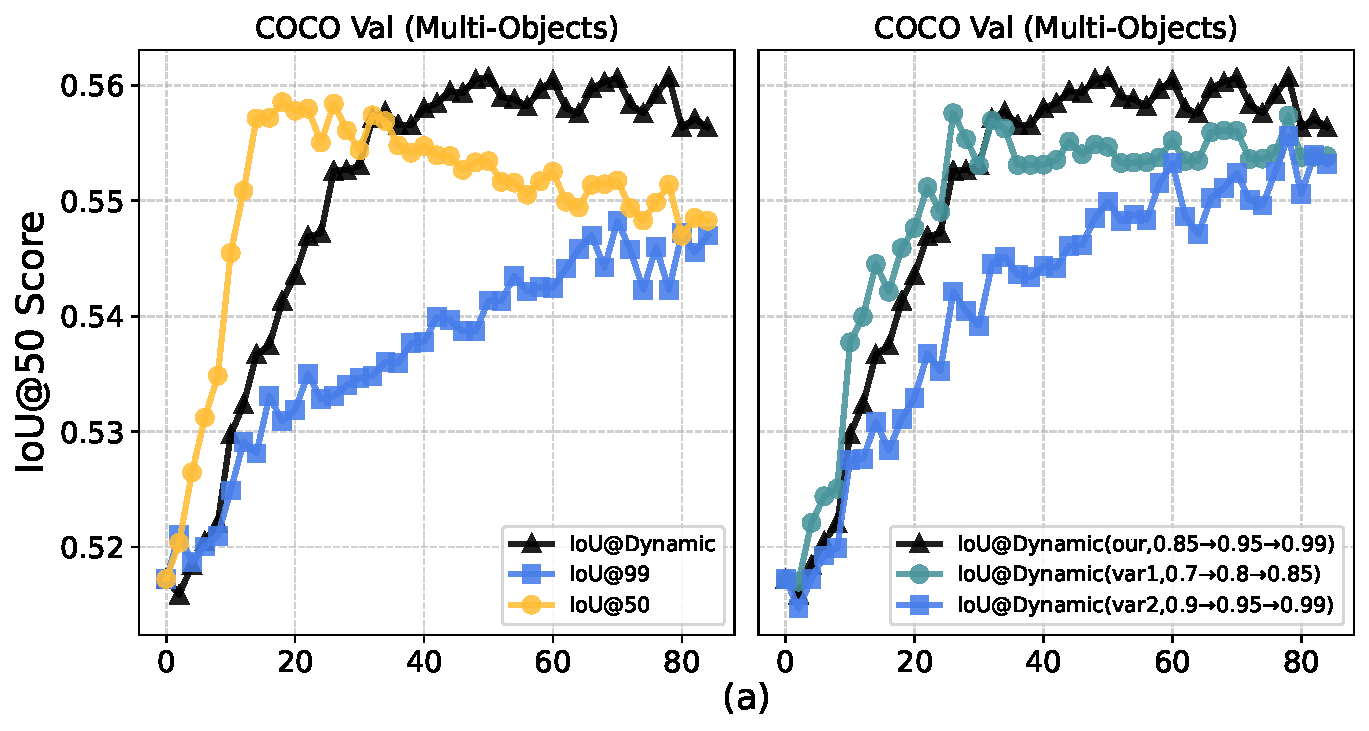
\includegraphics[width=0.98\linewidth]{figures/paper2/dynamic_iou.pdf}
    \end{column}
    \begin{column}{0.49\textwidth}
      \centering
      \tikz[baseline=(x.base)]\node[
        rounded corners=4pt,
        draw=red!55!black,
        fill=red!5,
        very thick,
        inner xsep=6pt,
        inner ysep=3pt,
        align=center
      ] (x) {\scriptsize Updating ViT causes gradient spikes};\\[0.50em]
      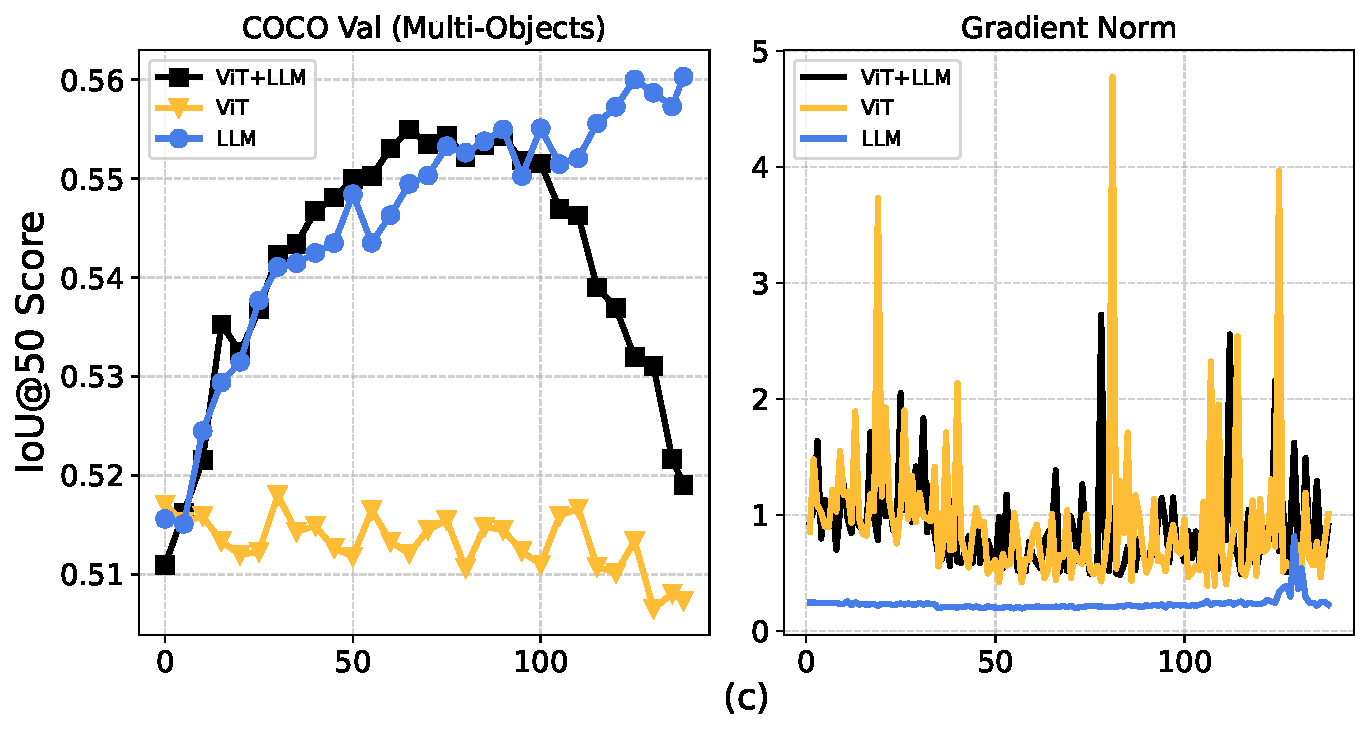
\includegraphics[width=0.98\linewidth]{figures/paper2/disable_vit.pdf}
    \end{column}
  \end{columns}

  \vspace{0.14cm}
  \begin{tikzpicture}[
    solution/.style={
      rounded corners=4pt,
      draw=green!45!black,
      fill=green!6,
      very thick,
      minimum width=4.60cm,
      minimum height=0.54cm,
      align=center,
      inner sep=2pt
    }
  ]
    \node[solution] at (-3.5,0) {\scriptsize Dynamic IoU: loose-to-strict localization curriculum};
    \node[solution] at (3.5,0) {\scriptsize Freezing ViT prevents perception degradation};
  \end{tikzpicture}

  \begin{flushright}
    {\fontsize{5.5}{5}\selectfont \textcolor{darkgray}{[2025.04-2025.06]~~\textit{One RL to See Them All: Visual Triple Unified Reinforcement Learning}, Ma et al.}}
  \end{flushright}
\end{frame}

\molochset{progressbar=foot}


\begin{frame}{\Large What Made Unified Multimodal RL Diagnosable?}
  \begin{columns}[T,onlytextwidth]
    \begin{column}{0.68\textwidth}
      \centering
      \vspace{0.35cm}
      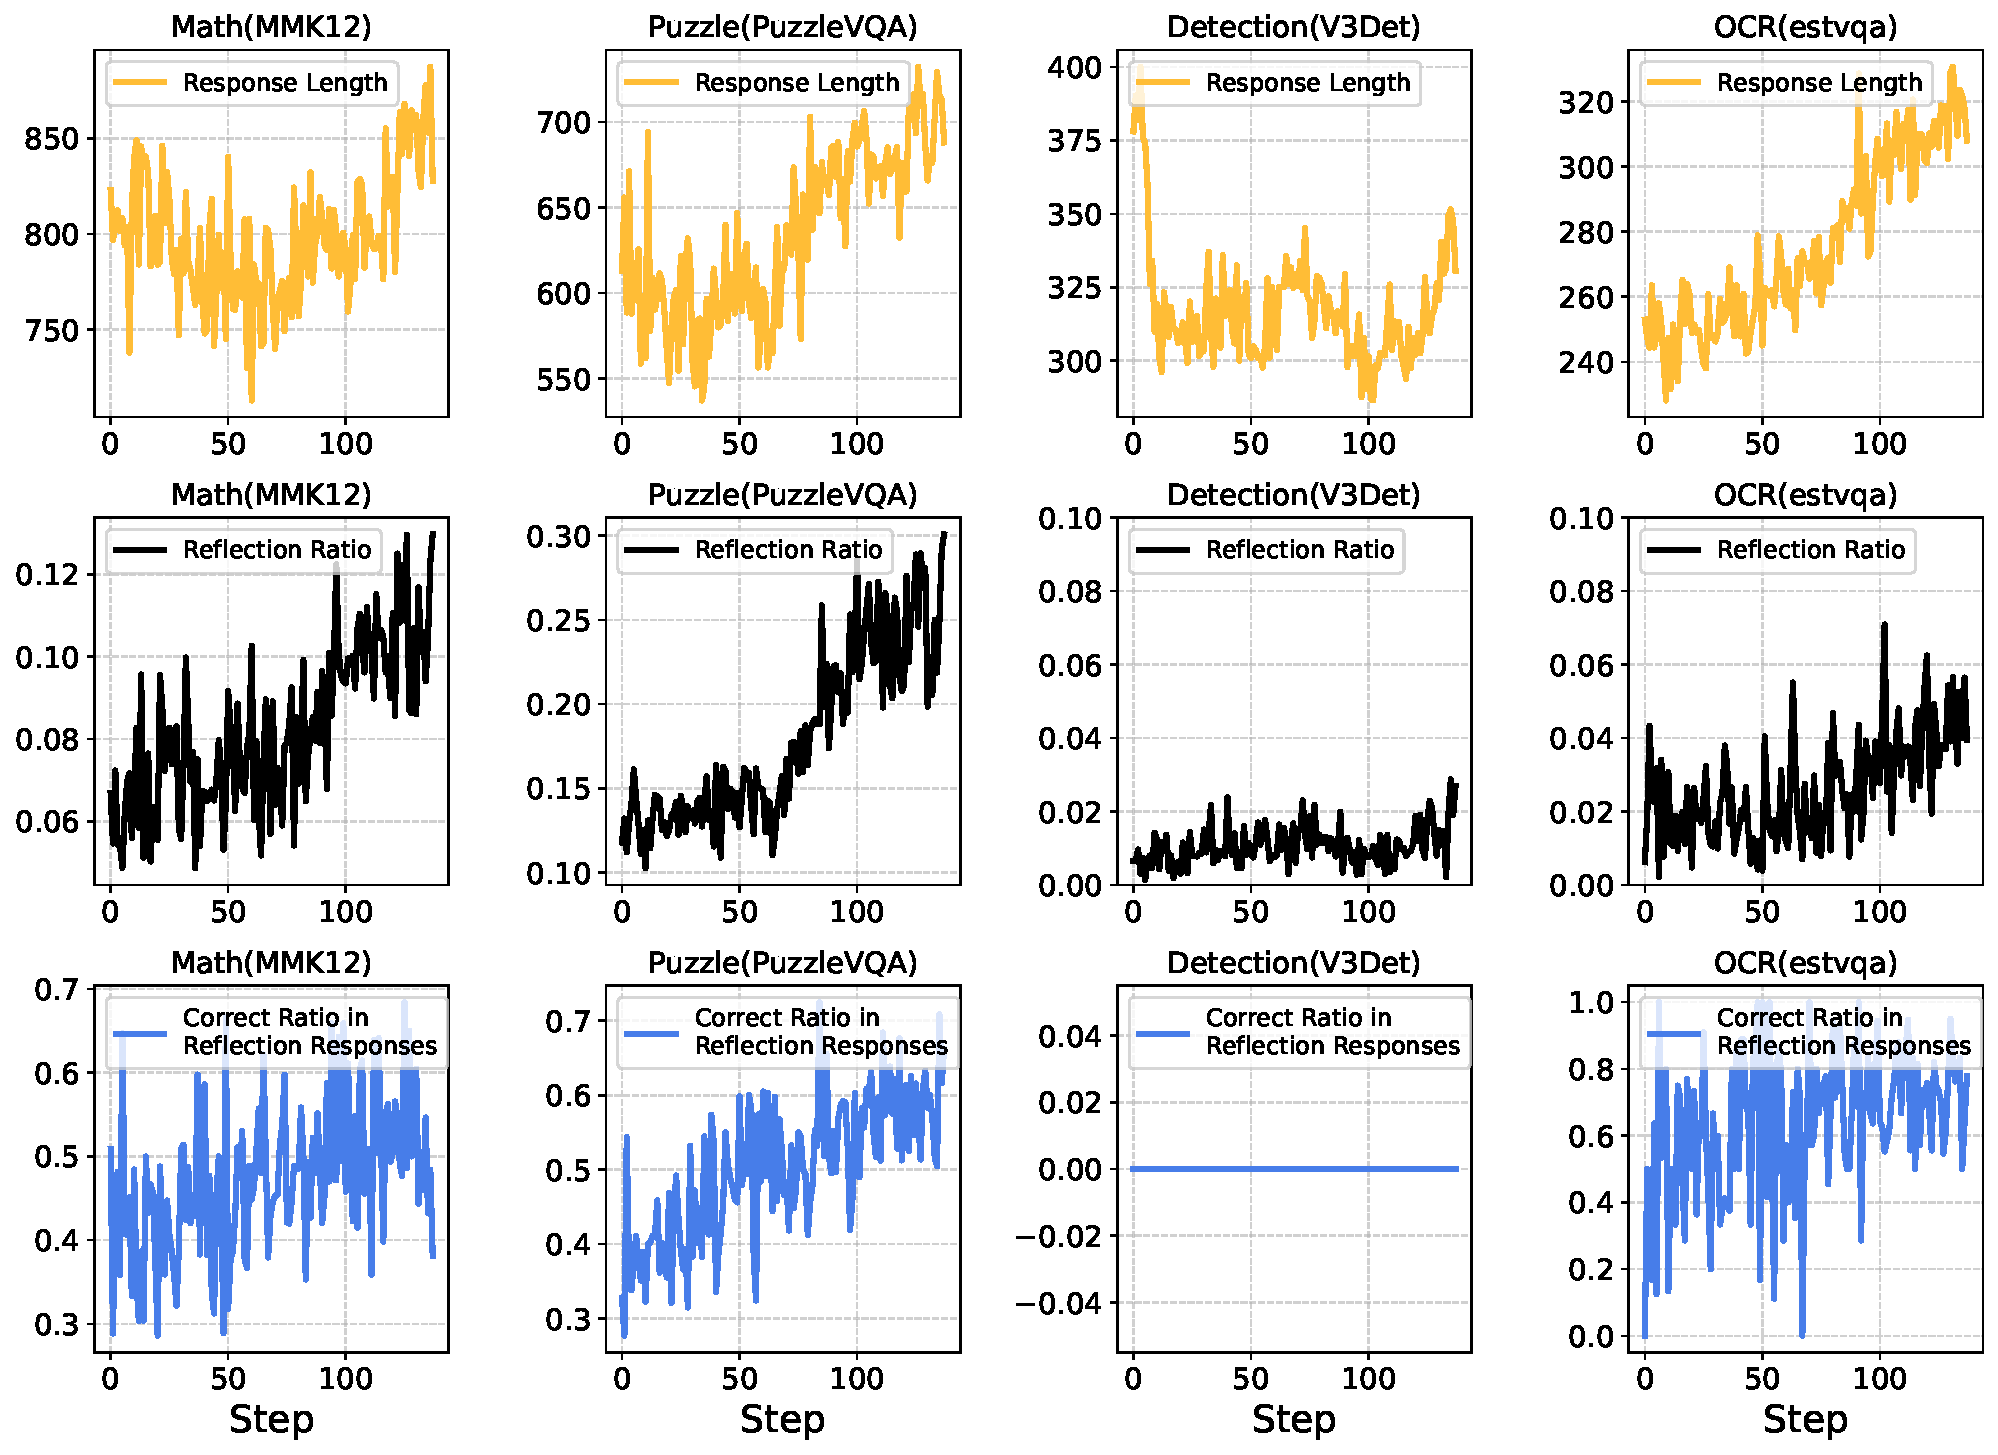
\includegraphics[width=0.98\linewidth]{figures/paper2/train_analysis.pdf}
    \end{column}
    \begin{column}{0.29\textwidth}
      \vspace{0.72cm}
      {\fontsize{8.5}{10}\selectfont Source diagnostics reveal task-specific behavior patterns hidden by aggregate metrics.}

      \vspace{0.42cm}
      \begin{tikzpicture}[
        insight/.style={
          rounded corners=4pt,
          draw=AgentBlueDark!45,
          fill=AgentGray,
          very thick,
          minimum width=3.95cm,
          minimum height=0.70cm,
          text width=3.85cm,
          align=center,
          inner sep=3pt
        }
      ]
        \node[insight] at (0,0) {\scriptsize Reasoning sources show length and reflection growth};
        \node[insight] at (0,-1.4) {\scriptsize Detection and OCR keep low-reflection patterns};
        \node[insight] at (0,-3.05) {\scriptsize Unified RL training preserves task-appropriate response styles};
      \end{tikzpicture}
    \end{column}
  \end{columns}

  \vspace{-0.14cm}
  \begin{flushright}
    {\fontsize{5.5}{5}\selectfont \textcolor{darkgray}{[2025.04-2025.06]~~\textit{One RL to See Them All: Visual Triple Unified Reinforcement Learning}, Ma et al.}}
  \end{flushright}
\end{frame}

\molochset{progressbar=foot}

\begin{frame}{\Large Can Unified Multimodal RL Scale with New Task Domains?}
  \centering
  \vspace{0.45cm}
  {\fontsize{11}{12}\selectfont Under a fixed-compute budget, unified training shows positive transfer when adding a new GUI grounding domain.}

  \vspace{0.35cm}
  \begingroup
  \setlength{\tabcolsep}{16pt}
  \renewcommand{\arraystretch}{1.20}
  {\small
  \begin{tabular}{@{}lcc@{}}
    \toprule
    Mixture & ScreenSpot-Pro & OCRBenchV2 \\
    \midrule
    Unified & 23.91 & 55.87 \\
    Perception-only & 23.78 & 55.33 \\
    Perception-only + GUI-3K & 29.85 & 55.96 \\
    Unified + GUI-3K & \textbf{31.68} & \textbf{56.09} \\
    \bottomrule
  \end{tabular}
  }
  \endgroup

  \vspace{0.35cm}
  \begin{tikzpicture}
    \node[
      rounded corners=4pt,
      draw=AgentBlueDark!45,
      fill=AgentGray,
      very thick,
      inner xsep=9pt,
      inner ysep=5pt,
      align=center
    ] {\scriptsize New-domain data improves ScreenSpot-Pro while OCRBenchV2 is preserved or slightly improved.};
  \end{tikzpicture}

  \vfill
  \begin{flushright}
    {\fontsize{5.5}{5}\selectfont \textcolor{darkgray}{[2025.04-2025.06]~~\textit{One RL to See Them All: Visual Triple Unified Reinforcement Learning}, Ma et al.}}
  \end{flushright}
\end{frame}

\molochset{progressbar=foot}

\begin{frame}{\Large From Perception + Reasoning to Acting Through Tools}
  \centering
  \vspace{-0.40cm}
  {\fontsize{11}{11}\selectfont
  Perception and reasoning operate on the current observation; vision tools let the model act to acquire new visual evidence.}

  \vspace{0.70cm}
  \begin{tikzpicture}[
    rootfade/.style={
      rounded corners=5pt,
      draw=AgentBlueDark!55,
      fill=AgentGray,
      very thick,
      minimum height=0.95cm,
      align=center,
      opacity=\SpotlightFadeOpacity,
      text opacity=\SpotlightFadeOpacity
    },
    activeouter/.style={
      rounded corners=5pt,
      draw=AgentBlueDark!75,
      fill=AgentGray,
      very thick,
      minimum width=4.15cm,
      minimum height=1.42cm,
      inner sep=0pt
    },
    fadeouter/.style={
      rounded corners=5pt,
      draw=AgentBlueDark!55,
      fill=AgentGray,
      very thick,
      minimum width=4.15cm,
      minimum height=1.42cm,
      inner sep=0pt,
      opacity=\SpotlightFadeOpacity
    },
    arrowfade/.style={-Latex,thick,draw=AgentBlueDark!80,opacity=\SpotlightFadeOpacity},
    arrowactive/.style={-Latex,thick,draw=AgentBlueDark!80},
    boundary/.style={thick,draw=AgentBlueDark!45,opacity=\SpotlightFadeOpacity}
  ]
    \node[rootfade,minimum width=1.8cm] (rl) at (-2.5,1.45) {\textbf{RL}};
    \node[rootfade,minimum width=3.7cm] (models) at (1.5,1.45) {\textbf{Multimodal Models \tiny(e.g. VLMs)}};
    \draw[arrowfade] (rl.east) -- (models.west);

    \node[fadeouter] (reason) at (-5.0,-0.80) {};
    \begin{scope}
      \clip[rounded corners=5pt] (reason.south west) rectangle (reason.north east);
      \fill[AgentBlue,opacity=\SpotlightFadeOpacity] (reason.north west) rectangle ([yshift=-0.50cm]reason.north east);
    \end{scope}
    \node[rounded corners=5pt,draw=AgentBlueDark!55,opacity=\SpotlightFadeOpacity,very thick,minimum width=4.15cm,minimum height=1.42cm,inner sep=0pt]
      at (reason.center) {};
    \node[minimum width=4.10cm,minimum height=0.50cm,anchor=north,inner sep=0pt,text opacity=\SpotlightFadeOpacity]
      at ([yshift=-0.03cm]reason.north) {\parbox{3.8cm}{\centering\fontsize{9}{9}\selectfont\bfseries Visual Reasoning}};
    \node[minimum width=4.10cm,minimum height=0.86cm,anchor=south,inner sep=0pt,text opacity=\SpotlightFadeOpacity]
      at ([yshift=0.03cm]reason.south) {\parbox{3.75cm}{\centering\fontsize{8.2}{10}\selectfont Reshapes training dynamics\\and improves generalization}};

    \node[fadeouter] (unified) at (0,-0.80) {};
    \begin{scope}
      \clip[rounded corners=5pt] (unified.south west) rectangle (unified.north east);
      \fill[AgentBlue,opacity=\SpotlightFadeOpacity] (unified.north west) rectangle ([yshift=-0.50cm]unified.north east);
    \end{scope}
    \node[rounded corners=5pt,draw=AgentBlueDark!55,opacity=\SpotlightFadeOpacity,very thick,minimum width=4.15cm,minimum height=1.42cm,inner sep=0pt]
      at (unified.center) {};
    \node[minimum width=4.10cm,minimum height=0.50cm,anchor=north,inner sep=0pt,text opacity=\SpotlightFadeOpacity]
      at ([yshift=-0.03cm]unified.north) {\parbox{3.8cm}{\centering\fontsize{9}{9}\selectfont\bfseries Perception + Reasoning}};
    \node[minimum width=4.10cm,minimum height=0.86cm,anchor=south,inner sep=0pt,text opacity=\SpotlightFadeOpacity]
      at ([yshift=0.03cm]unified.south) {\parbox{3.75cm}{\centering\fontsize{8.2}{10}\selectfont Positive transfer under joint\\multimodal RL training}};

    \node[activeouter] (tool) at (5.0,-0.80) {};
    \begin{scope}
      \clip[rounded corners=5pt] (tool.south west) rectangle (tool.north east);
      \fill[AgentBlue] (tool.north west) rectangle ([yshift=-0.50cm]tool.north east);
    \end{scope}
    \node[rounded corners=5pt,draw=AgentBlueDark!75,very thick,minimum width=4.15cm,minimum height=1.42cm,inner sep=0pt]
      at (tool.center) {};
    \node[minimum width=4.10cm,minimum height=0.50cm,anchor=north,inner sep=0pt]
      at ([yshift=-0.03cm]tool.north) {\parbox{3.8cm}{\centering\fontsize{9}{9}\selectfont\bfseries Vision Tool-Use}};
    \node[minimum width=4.10cm,minimum height=0.86cm,anchor=south,inner sep=0pt]
      at ([yshift=0.03cm]tool.south) {\parbox{3.75cm}{\centering\fontsize{8.2}{10}\selectfont Intrinsic learning dominates\\RL reduces tool-induced harm}};

    \draw[boundary] (rl.south west) to[out=235,in=75] (reason.north west);
    \draw[boundary] (models.south east) to[out=-45,in=105] (tool.north east);
    \draw[arrowfade] (reason.east) -- (unified.west);
    \draw[arrowactive] (unified.east) -- (tool.west);
  \end{tikzpicture}

  \vspace{0.55cm}
  {\fontsize{10.5}{12}\selectfont
  \textbf{Next question:} what does RL actually learn when the model can act through visual tools?}
\end{frame}

\molochset{progressbar=foot}

\begin{frame}{\Large How Can We Disentangle What Vision Tool-Use RL Learns?}
  \centering
  \vspace{0.12cm}
  {\fontsize{9}{10.5}\selectfont MED is a coarse-to-fine analysis framework for tracking both intrinsic model changes and tool-induced outcome changes during vision tool-use RL.}

  \vspace{0.25cm}
  \includegraphics[width=0.80\linewidth]{figures/paper3/med_framework.pdf}

  \vspace{-0.25cm}
  \begin{flushright}
    {\fontsize{5.5}{5}\selectfont \textcolor{darkgray}{[2025.10-2026.01]~~\textit{What Does Vision Tool-Use Reinforcement Learning Really Learn? Disentangling Tool-Induced and Intrinsic Effects for Crop-and-Zoom}, Ma et al.}}
  \end{flushright}
\end{frame}

\molochset{progressbar=foot}

\begin{frame}{\Large How Can We Disentangle What Vision Tool-Use RL Learns?}
  \centering
  \vspace{0.35cm}
  \begin{tikzpicture}
    \node[anchor=south west,inner sep=0pt] (medfig) at (0,0)
      {\includegraphics[width=0.95\linewidth]{figures/paper3/med_framework.pdf}};
    \begin{scope}[x={(medfig.south east)},y={(medfig.north west)}]
      \filldraw[
        rounded corners=2pt,
        fill=white,
        fill opacity=0.95,
        draw=AgentBlueDark!25,
        line width=0.5pt
      ] (0.265,0.02) rectangle (0.999,0.985);
      \node[
        anchor=north west,
        align=left,
        text width=0.66\linewidth
      ] at (0.305,0.95) {%
        \fontsize{6.7}{8.1}\selectfont
        {\fontsize{8.0}{9.2}\selectfont\textbf{a) Vision tool-use RL training \& evaluation}}\\[0.25em]
        A VLM $\Phi$ is trained with RL; during decoding, it may call a visual tool.\\[0.35em]
        At each checkpoint $t\in[0,T]$, evaluate two protocols:\\[-0.30em]
        \[
          Acc_{\mathrm{wo}}(t): \text{tool-free}, \qquad
          Acc_{\mathrm{w}}(t): \text{tool-available}
        \]
        \vspace{-1.05em}
        Tool-induced performance gap at checkpoint $t$:\\[0.15em]
        \[
          G(t)=Acc_{\mathrm{w}}(t)-Acc_{\mathrm{wo}}(t)
        \]
      };
      \node[
        anchor=north west,
        align=left,
        text width=0.66\linewidth
      ] at (0.305,0.42) {%
        \fontsize{6.7}{8.1}\selectfont
        {\fontsize{8.0}{9.2}\selectfont\textbf{b) Measure: quantifying tool-induced drift}}\\[-0.15em]
        \[
          f_{\mathrm{wo}}(t)=Acc_{\mathrm{wo}}(t)-Acc_{\mathrm{wo}}(0), \quad
          f_{\mathrm{w}}(t)=Acc_{\mathrm{w}}(t)-Acc_{\mathrm{w}}(0)
        \]
        \vspace{-1.05em}
        \[
          \Delta_{\mathrm{tool}}(t)=G(t)-G(0)
        \]
        \vspace{-1.05em}
        \[
          \underbrace{f_{\mathrm{w}}(t)}_{\text{Tool-available drift}}
          =
          \underbrace{f_{\mathrm{wo}}(t)}_{\text{Intrinsic drift}}
          +
          \underbrace{\Delta_{\mathrm{tool}}(t)}_{\text{Tool-induced drift}}
        \]
      };
    \end{scope}
  \end{tikzpicture}

  \vspace{-0.25cm}
  \begin{flushright}
    {\fontsize{5.5}{5}\selectfont \textcolor{darkgray}{[2025.10-2026.01]~~\textit{What Does Vision Tool-Use Reinforcement Learning Really Learn? Disentangling Tool-Induced and Intrinsic Effects for Crop-and-Zoom}, Ma et al.}}
  \end{flushright}
\end{frame}

\molochset{progressbar=foot}

\begin{frame}{\Large How Can We Disentangle What Vision Tool-Use RL Learns?}
  \centering
  \vspace{0.35cm}
  \begin{tikzpicture}
    \node[anchor=south west,inner sep=0pt] (medfig) at (0,0)
      {\includegraphics[width=0.95\linewidth]{figures/paper3/med_framework.pdf}};
    \begin{scope}[x={(medfig.south east)},y={(medfig.north west)}]
      \filldraw[
        rounded corners=2pt,
        fill=white,
        fill opacity=0.95,
        draw=AgentBlueDark!25,
        line width=0.5pt
      ] (0.000,0.02) rectangle (0.265,0.985);
      \node[
        anchor=north west,
        align=left,
        text width=0.255\linewidth
      ] at (-0.01,0.98) {%
        \fontsize{8}{11}\selectfont
        {\fontsize{5}{4}\selectfont\textbf{c) Explain: decompose tool-induced gap}}\\[0.12em]
        \par\vspace{0.50em}\noindent
        \resizebox{0.98\linewidth}{!}{$
          \begin{aligned}
          & G(t) = Acc_{\mathrm{w}}(t)-Acc_{\mathrm{wo}}(t) \\
          & =\underbrace{P(\mathcal D_{\text{fail}}) P(c \mid \mathcal D_{\text{fail}}) P(\checkmark \mid c, \mathcal D_{\text{fail}})}_{\text{Term 1: Call Gain}} \\
          & +\underbrace{P(\mathcal D_{\text{fail}}) P(\neg c \mid \mathcal D_{\text{fail}}) P(\checkmark \mid \neg c, \mathcal D_{\text{fail}})}_{\text{Term 2: Schema Gain}} \\
          & -\underbrace{P(\mathcal D_{\text{succ}}) P(c \mid \mathcal D_{\text{succ}}) P(\times \mid c, \mathcal D_{\text{succ}})}_{\text{Term 3: Call Harm}} \\
          & -\underbrace{P(\mathcal D_{\text{succ}}) P(\neg c \mid \mathcal D_{\text{succ}}) P(\times \mid \neg c, \mathcal D_{\text{succ}})}_{\text{Term 4: Schema Harm}}
          \end{aligned}
        $}
        \par\vspace{2.55em}
        {\fontsize{6}{6}\selectfont\textbf{d) Diagnose: factorize each term}}\\[0.20em]
        \resizebox{0.98\linewidth}{!}{$
          \mathrm{Term}(\mathcal D,a,o)
          =
          \underbrace{P(\mathcal D)}_{\text{Mass}}
          \cdot
          \underbrace{P(a\mid\mathcal D)}_{\text{Policy}}
          \cdot
          \underbrace{P(o\mid a,\mathcal D)}_{\text{Quality}}
        $}
      };
    \end{scope}
  \end{tikzpicture}

  \vspace{-0.25cm}
  \begin{flushright}
    {\fontsize{5.5}{5}\selectfont \textcolor{darkgray}{[2025.10-2026.01]~~\textit{What Does Vision Tool-Use Reinforcement Learning Really Learn? Disentangling Tool-Induced and Intrinsic Effects for Crop-and-Zoom}, Ma et al.}}
  \end{flushright}
\end{frame}

\molochset{progressbar=foot}

\begin{frame}{\Large Do Gains Come From Tool Use or Intrinsic Learning?}
  \begin{columns}[T,onlytextwidth]
    \begin{column}{0.67\textwidth}
      \centering
      % \vspace{0.33cm}
      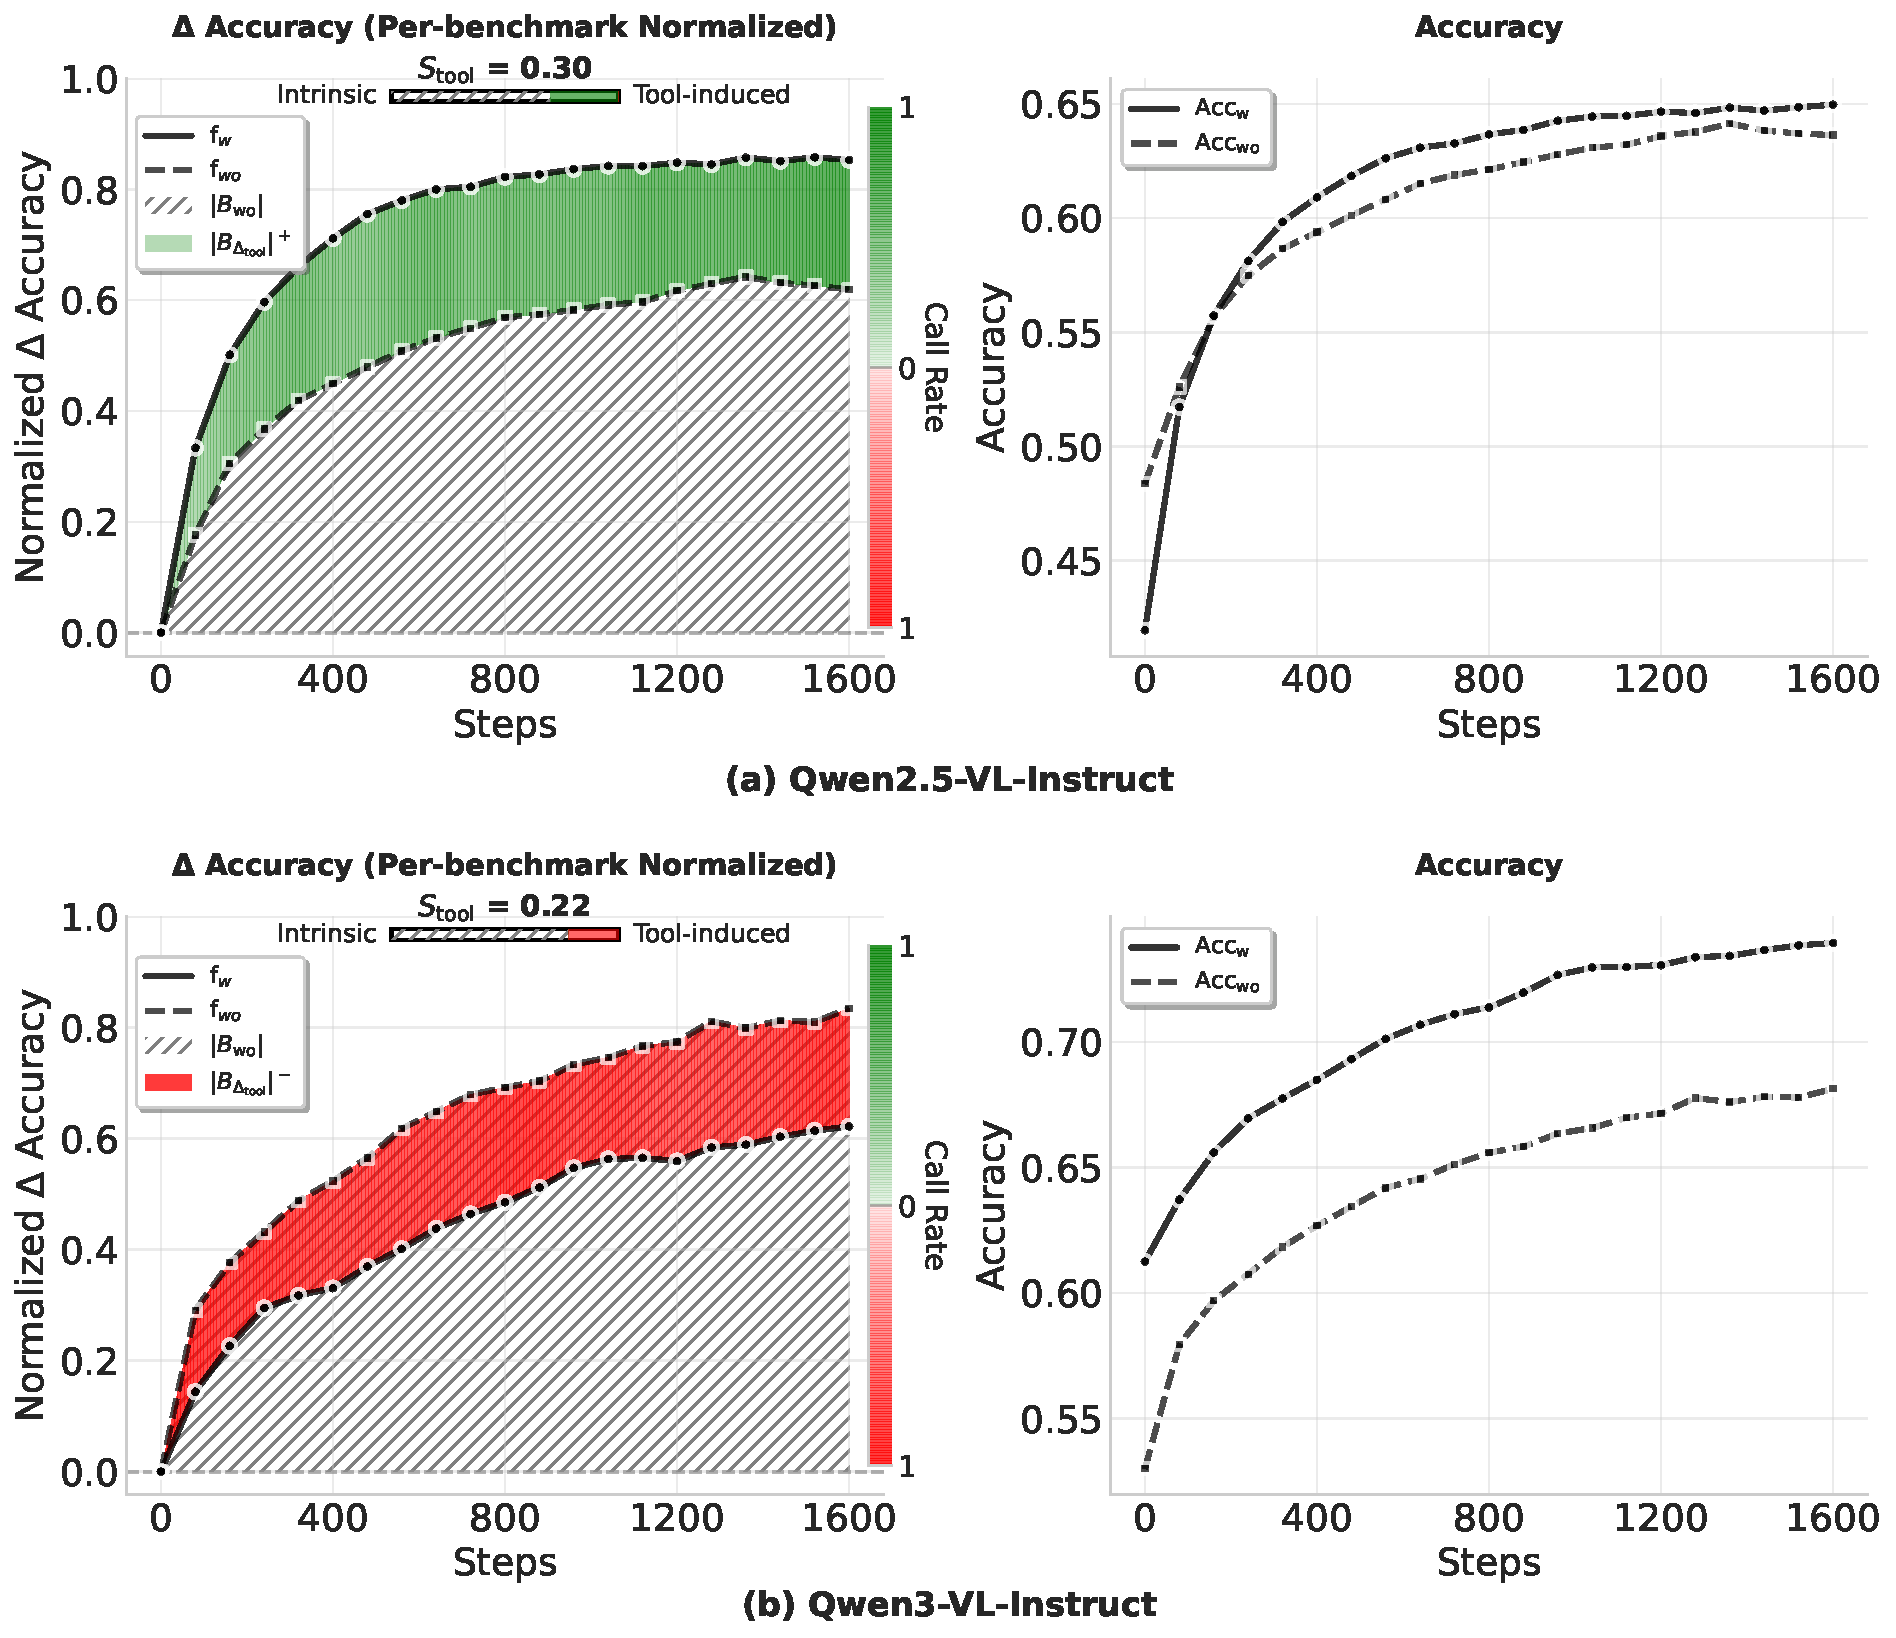
\includegraphics[width=0.90\linewidth]{figures/paper3/exp1_intrinsic_tool_drift.pdf}
    \end{column}
    \begin{column}{0.32\textwidth}
      \vspace{0.18cm}
      \newcommand{\intrinsicarea}{%
        \tikz[baseline=-0.45ex]{
          \fill[gray!28] (0,0) rectangle (0.30,0.15);
          \draw[gray!70,line width=0.25pt] (0.02,0) -- (0.17,0.15);
          \draw[gray!70,line width=0.25pt] (0.11,0) -- (0.26,0.15);
          \draw[gray!70,line width=0.25pt] (0.20,0) -- (0.30,0.10);
        }%
      }
      \newcommand{\toolareas}{%
        \tikz[baseline=-0.45ex]{
          \fill[green!35!white] (0,0) rectangle (0.13,0.15);
          \fill[red!35!white] (0.17,0) rectangle (0.30,0.15);
          \draw[gray!55,line width=0.25pt] (0,0) rectangle (0.13,0.15);
          \draw[gray!55,line width=0.25pt] (0.17,0) rectangle (0.30,0.15);
        }%
      }
      \setlength{\leftmargini}{1.05em}
      {\fontsize{7.0}{8.4}\selectfont
      \textbf{Setup}
      \begin{itemize}
        \setlength{\itemsep}{0.50em}
        \item Crop-and-Zoom-in tool.
        \item $\sim$15K high-resolution samples.
        \item Only 0-1 final-answer reward.
        \item Checkpoint evaluation w vs. w/o tool access on 6 benchmarks.
        \item Qwen2.5-VL vs. Qwen3-VL (7B): different tool prior.
      \end{itemize}
      }

      \vspace{0.10cm}
      {\fontsize{7.8}{9.4}\selectfont
      \textbf{Findings}
      \begin{itemize}
        \setlength{\itemsep}{0.60em}
        \item Intrinsic drift dominates: \\[0.15em] \intrinsicarea{} $>$ \toolareas{}; $S_{\mathrm{tool}}=0.30/0.22$.
        \item Different tool priors lead to different tool-induced drift.
        \item Both tool-free and tool-available accuracy improve (right fig).
      \end{itemize}
      }
    \end{column}
  \end{columns}

  \begin{flushright}
    \vspace{-0.18cm}
    {\fontsize{5.5}{5}\selectfont \textcolor{darkgray}{[2025.10-2026.01]~~\textit{What Does Vision Tool-Use Reinforcement Learning Really Learn? Disentangling Tool-Induced and Intrinsic Effects for Crop-and-Zoom}, Ma et al.}}
  \end{flushright}
\end{frame}

\molochset{progressbar=foot}

\begin{frame}{\Large Does Vision Tool-Use RL Expand Gain or Reduce Harm?}
  \centering
  \vspace{0.03cm}
  {\fontsize{9.5}{10}\selectfont Tool-use RL mainly reduces tool-induced harm rather than continuously increasing tool-based gain.}

  \vspace{0.16cm}
  \begin{columns}[T,onlytextwidth]
    \begin{column}{0.49\textwidth}
      \centering
      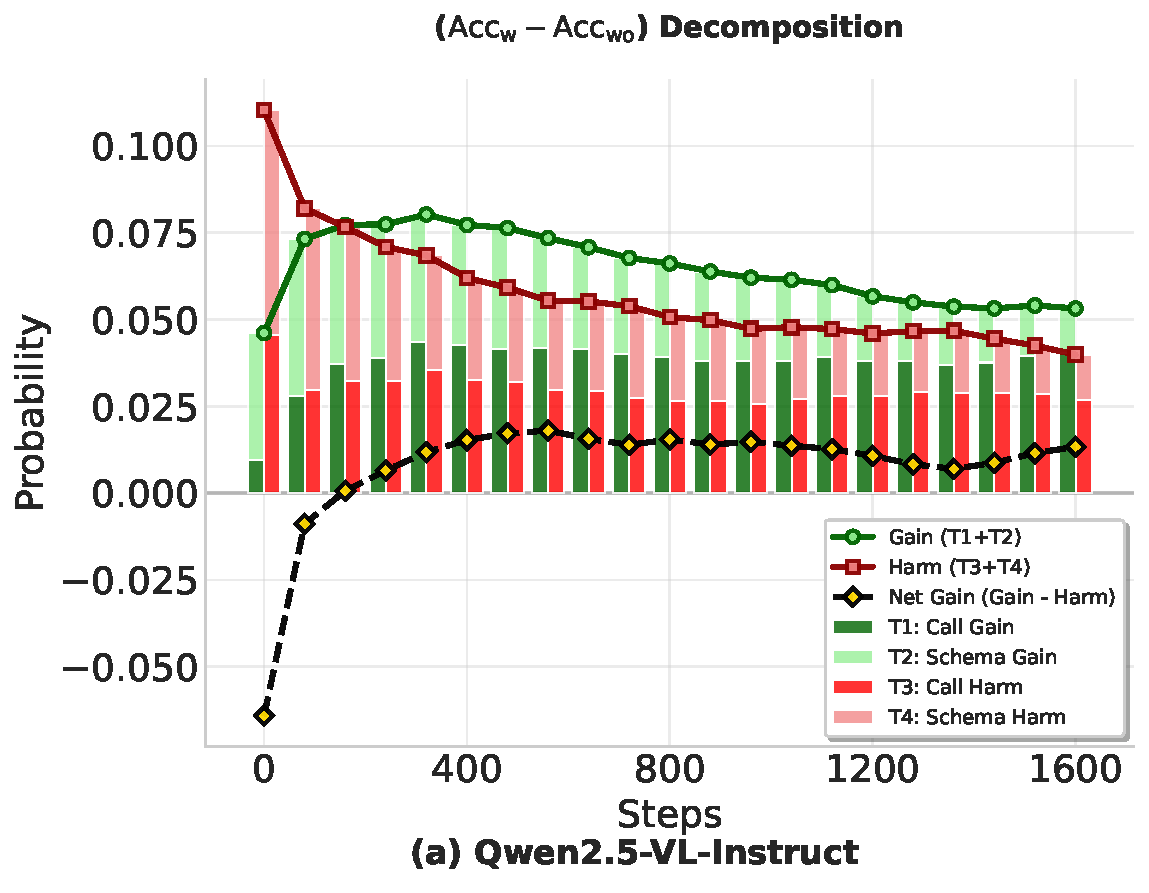
\includegraphics[width=0.98\linewidth]{figures/paper3/exp2_gain_harm_1.pdf}
    \end{column}
    \begin{column}{0.49\textwidth}
      \centering
      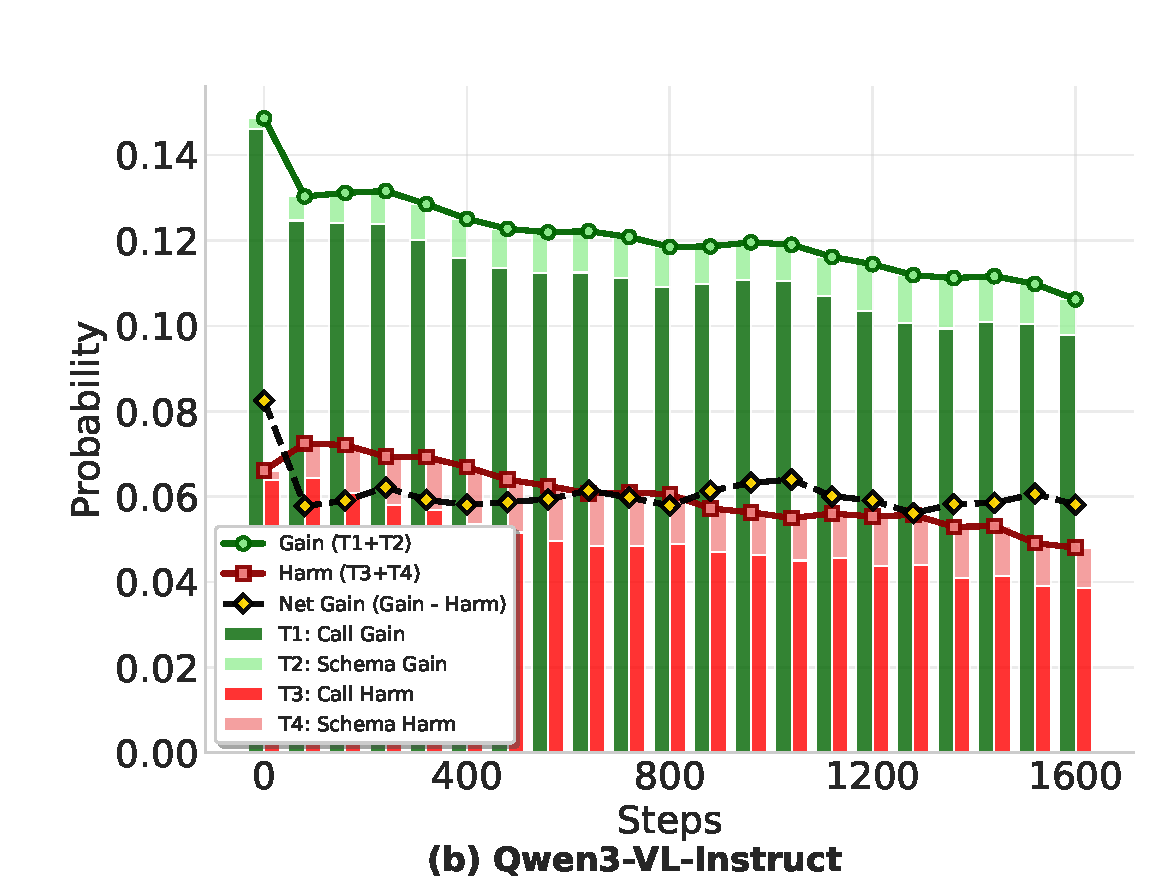
\includegraphics[width=0.98\linewidth]{figures/paper3/exp2_gain_harm_2.pdf}
    \end{column}
  \end{columns}

  \vspace{0.10cm}
  \begin{tikzpicture}[
    takeaway/.style={
      rounded corners=4pt,
      very thick,
      minimum width=4.30cm,
      minimum height=0.54cm,
      align=center,
      inner sep=2pt
    }
  ]
    \node[takeaway,draw=green!45!black,fill=green!6] at (-2.3,0) {\scriptsize Gross gain saturates or declines};
    \node[takeaway,draw=red!55!black,fill=red!5] at (5.0,0) {\scriptsize Gross harm consistently decreases};
  \end{tikzpicture}

  \begin{flushright}
    \vspace{-0.06cm}
    {\fontsize{5.5}{5}\selectfont \textcolor{darkgray}{[2025.10-2026.01]~~\textit{What Does Vision Tool-Use Reinforcement Learning Really Learn? Disentangling Tool-Induced and Intrinsic Effects for Crop-and-Zoom}, Ma et al.}}
  \end{flushright}
\end{frame}

\molochset{progressbar=foot}

\begin{frame}{\Large Why Does Tool Gain Remain Limited?}
  \centering
  \vspace{0.04cm}
  {\fontsize{9.0}{10.5}\selectfont Factor analysis suggests RL suppresses tool-related mistakes more than it improves correction.}

  \vspace{0.10cm}
  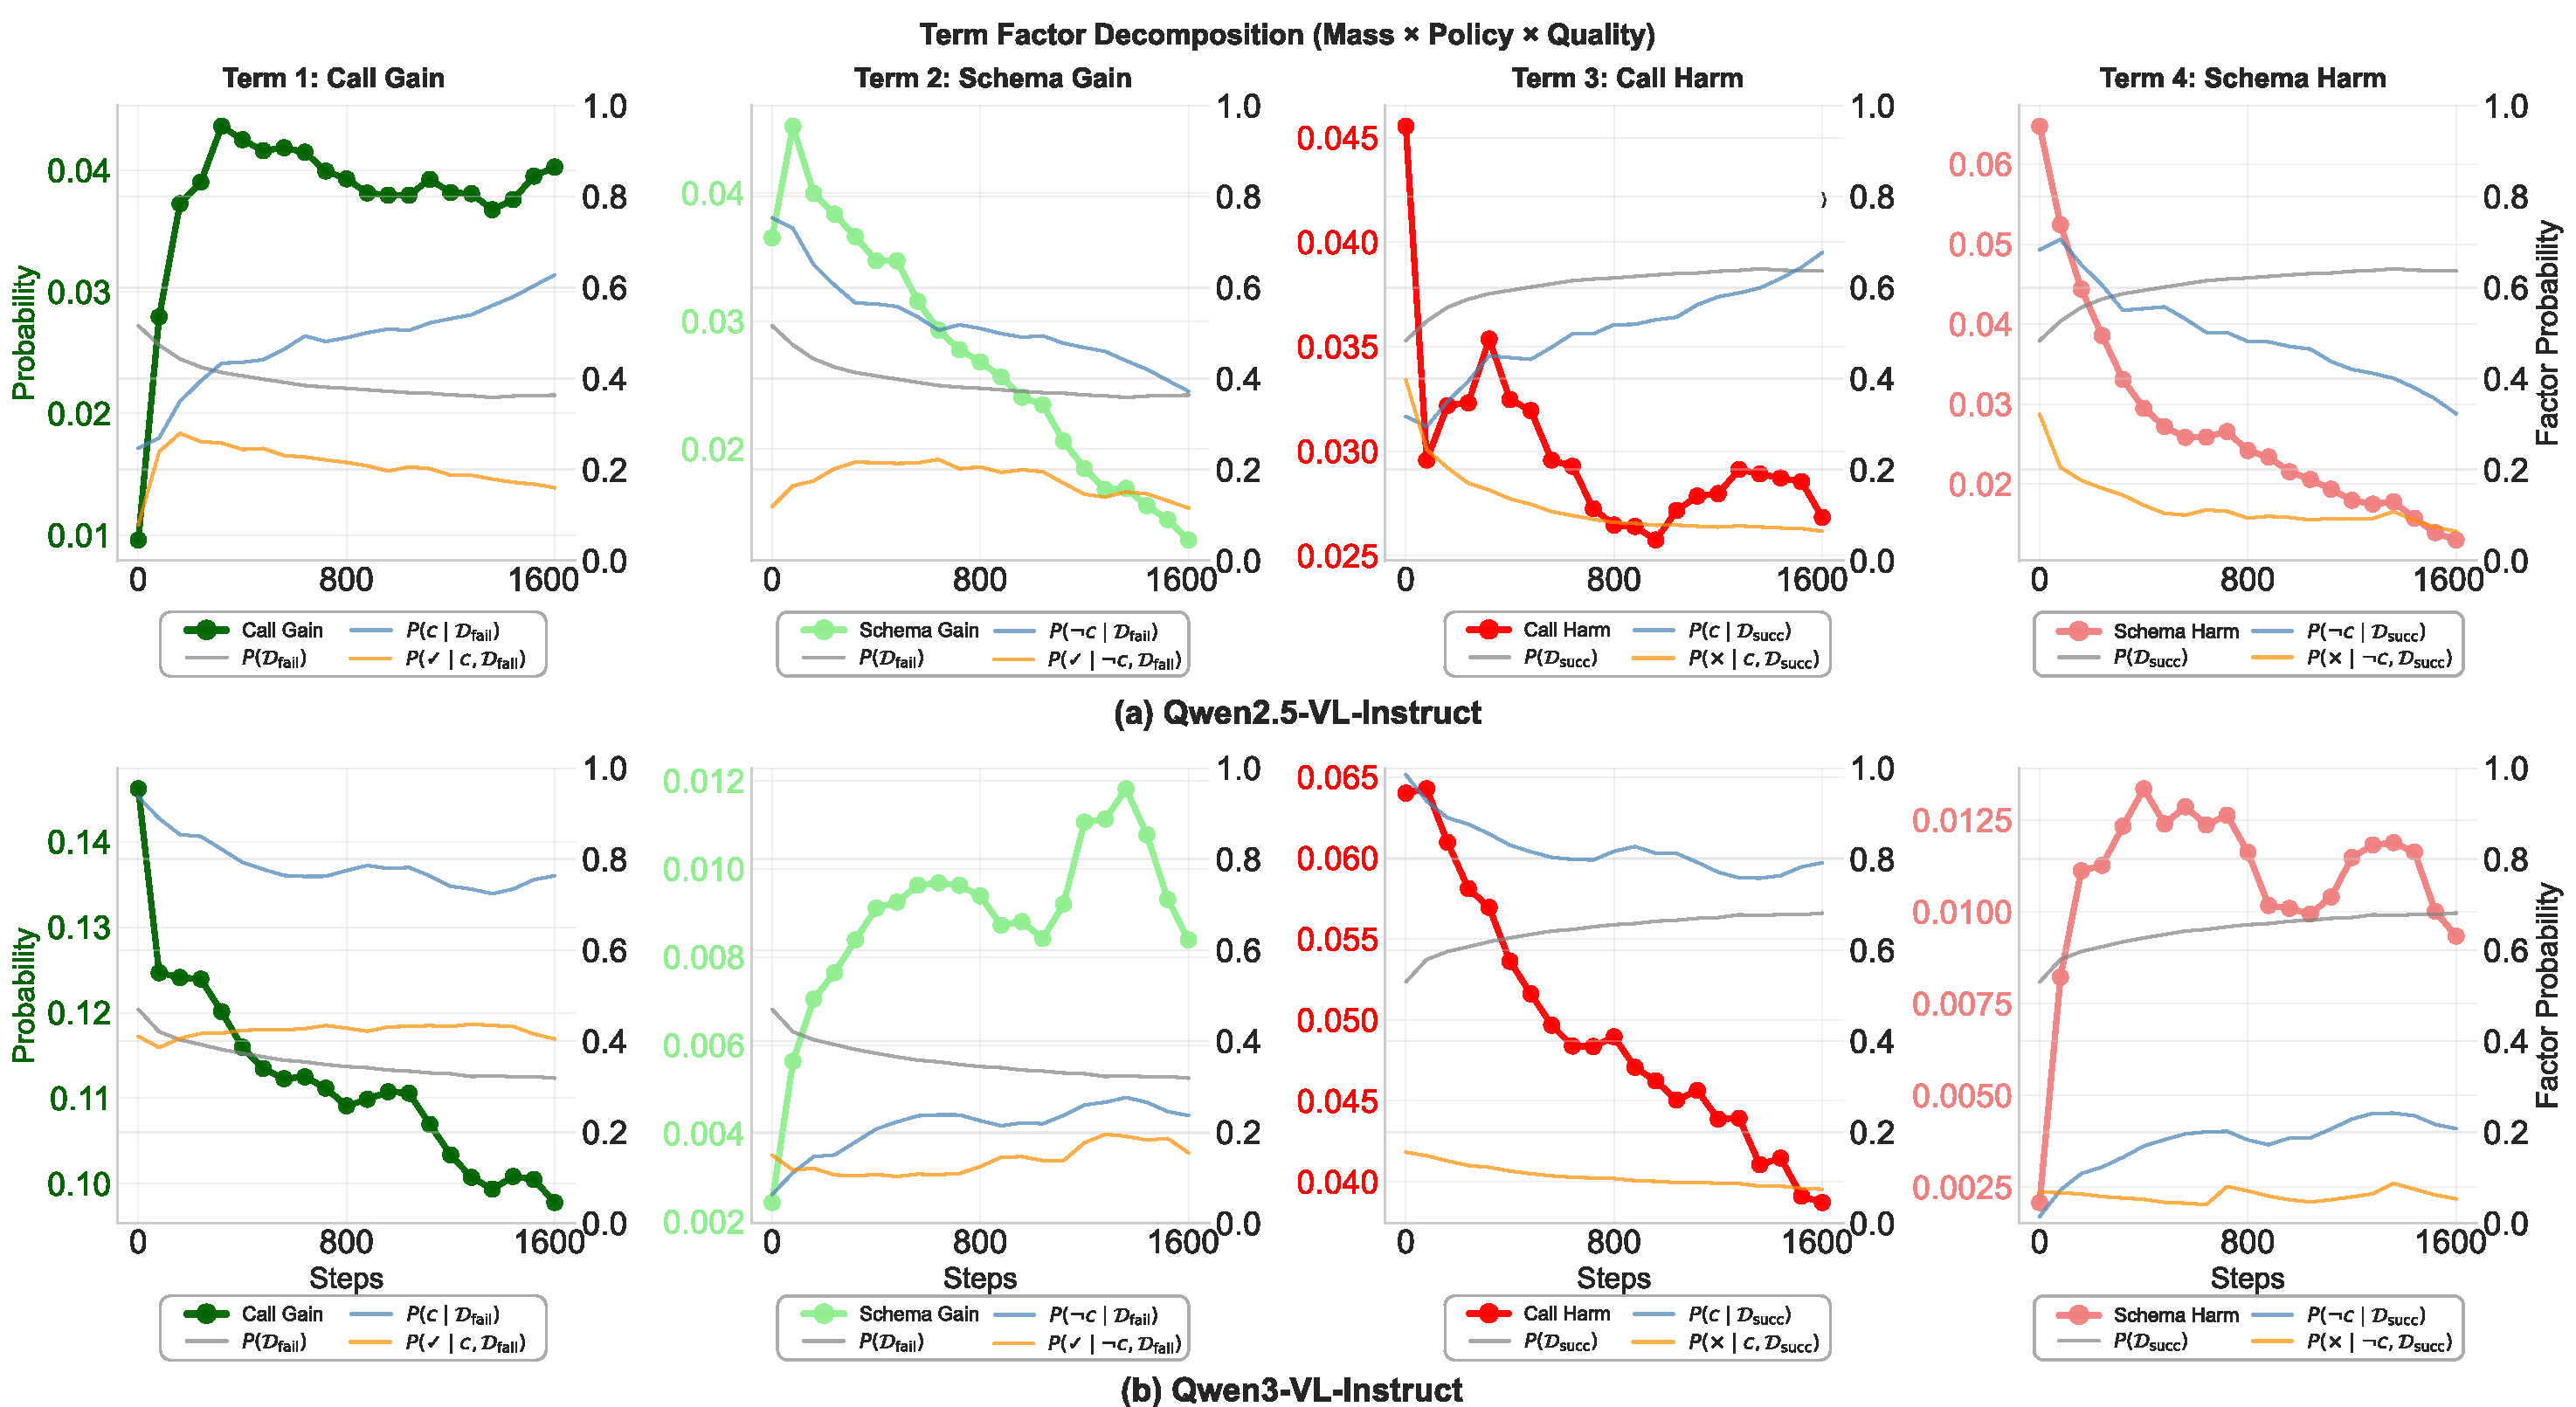
\includegraphics[width=0.85\linewidth]{figures/paper3/exp3_factor_decomposition.pdf}

  \vspace{-0.18cm}
  \begin{flushright}
    {\fontsize{5.5}{5}\selectfont \textcolor{darkgray}{[2025.10-2026.01]~~\textit{What Does Vision Tool-Use Reinforcement Learning Really Learn? Disentangling Tool-Induced and Intrinsic Effects for Crop-and-Zoom}, Ma et al.}}
  \end{flushright}
\end{frame}

\molochset{progressbar=foot}

\begin{frame}{\Large Diagnose I: Tool Calls, Gain vs. Harm}
  \centering
  \vspace{0.12cm}
  \begin{tikzpicture}
    \node[anchor=south west,inner sep=0pt] (expthree) at (0,0)
      {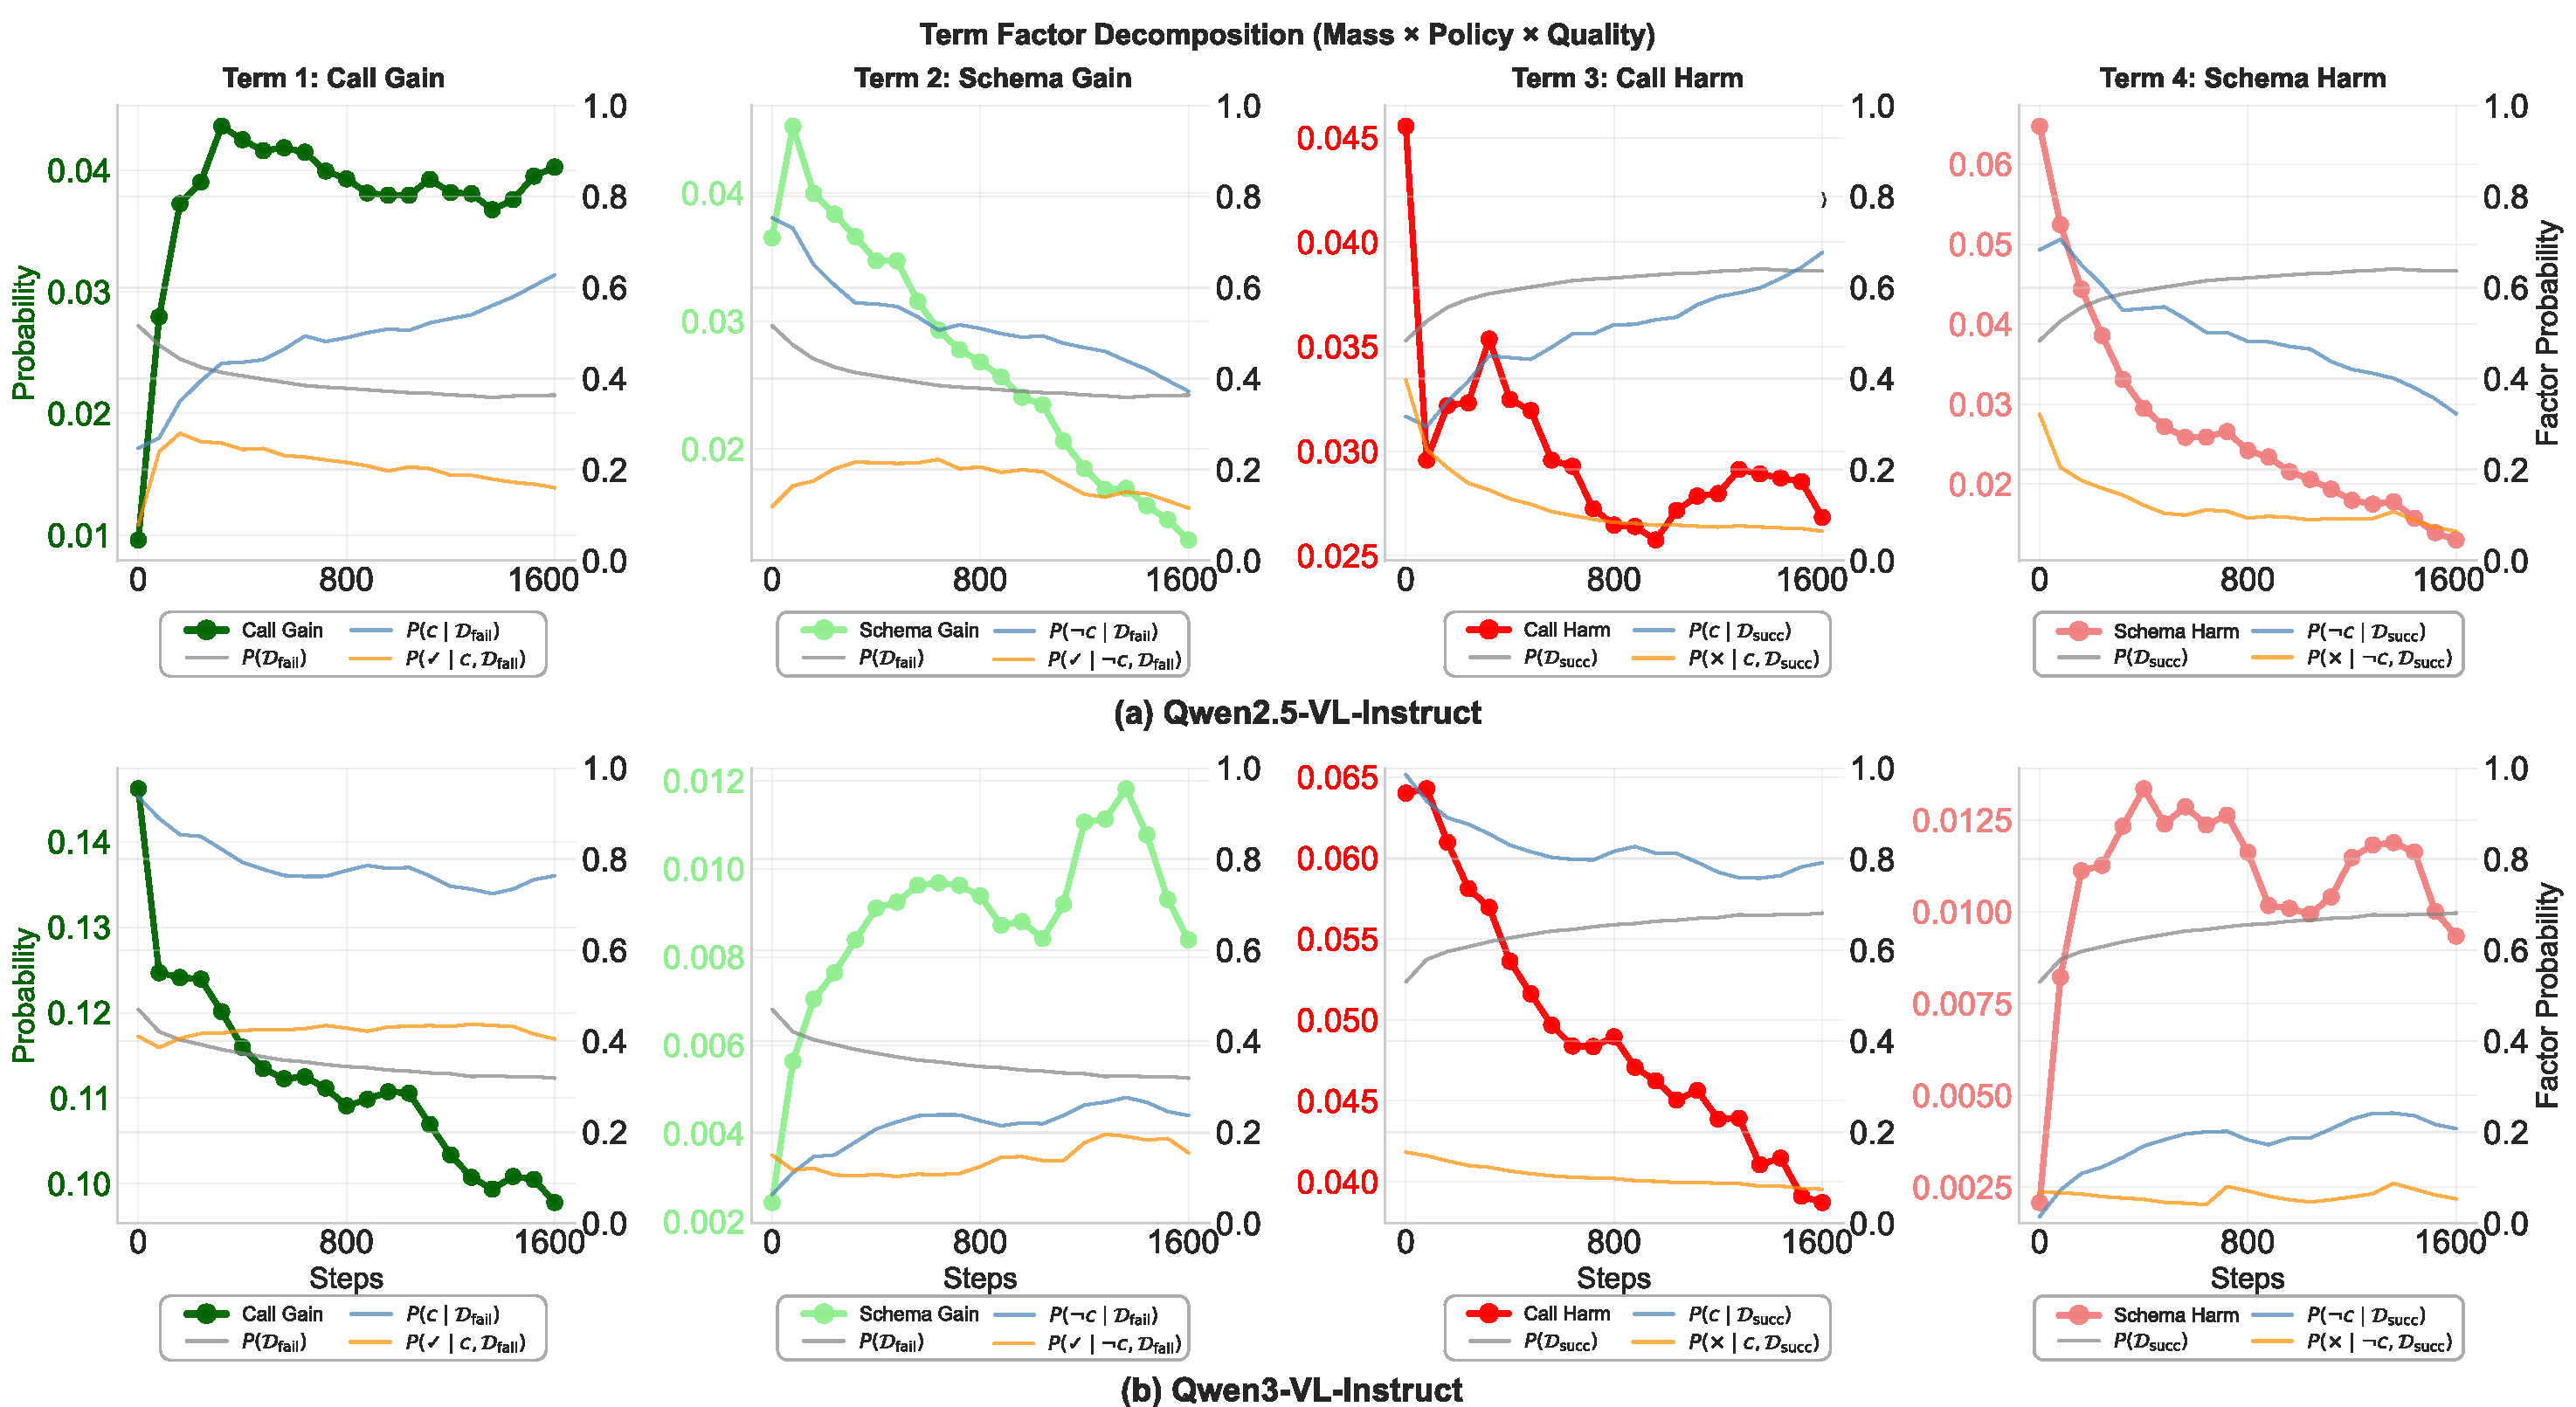
\includegraphics[width=0.98\linewidth]{figures/paper3/exp3_factor_decomposition.pdf}};
    \begin{scope}[x={(expthree.south east)},y={(expthree.north west)}]
      \filldraw[
        fill=white,
        fill opacity=0.95,
        draw=none
      ] (0.255,0.02) rectangle (0.495,0.935);
      \filldraw[
        fill=white,
        fill opacity=0.95,
        draw=none
      ] (0.74,0.02) rectangle (0.995,0.935);
      \node[
        text width=0.225\linewidth,
        align=left,
        inner sep=0pt
      ] at (0.375,0.75) {%
        {\fontsize{5.9}{6.8}\selectfont
        \textcolor{green!40!black}{\textbf{Qwen2.5-VL: \\ T1 Call Gain} $\uparrow\text{-}\to$}
        $=$
        \textcolor{gray}{$P(\mathcal D_{\mathrm{fail}})\downarrow$}
        $\times$
        \textcolor{SteelBlue}{$P(c|\mathcal D_{\mathrm{fail}})\uparrow$}
        $\times$
        \textcolor{DarkOrange}{$P(\checkmark|c,\mathcal D_{\mathrm{fail}})\uparrow\text{-}\downarrow$}}
      };
      \node[
        text width=0.225\linewidth,
        align=left,
        inner sep=0pt
      ] at (0.865,0.75) {%
        {\fontsize{5.9}{6.8}\selectfont
        \textcolor{red!75!black}{\textbf{Qwen2.5-VL: \\ T3 Call Harm} $\downarrow$}
        $=$
        \textcolor{gray}{$P(\mathcal D_{\mathrm{succ}})\uparrow$}
        $\times$
        \textcolor{SteelBlue}{$P(c|\mathcal D_{\mathrm{succ}})\uparrow$}
        $\times$
        \textcolor{DarkOrange}{$P(\times|c,\mathcal D_{\mathrm{succ}})\downarrow$}}
      };
      \node[
        text width=0.225\linewidth,
        align=left,
        inner sep=0pt
      ] at (0.375,0.28) {%
        {\fontsize{5.9}{6.8}\selectfont
        \textcolor{green!40!black}{\textbf{Qwen3-VL: \\ T1 Call Gain} $\downarrow$}
        $=$
        \textcolor{gray}{$P(\mathcal D_{\mathrm{fail}})\downarrow$}
        $\times$
        \textcolor{SteelBlue}{$P(c|\mathcal D_{\mathrm{fail}})\downarrow$}
        $\times$
        \textcolor{DarkOrange}{$P(\checkmark|c,\mathcal D_{\mathrm{fail}})\to$}}
      };
      \node[
        text width=0.225\linewidth,
        align=left,
        inner sep=0pt
      ] at (0.865,0.28) {%
        {\fontsize{5.9}{6.8}\selectfont
        \textcolor{red!75!black}{\textbf{Qwen3-VL: \\ T3 Call Harm} $\downarrow$}
        $=$
        \textcolor{gray}{$P(\mathcal D_{\mathrm{succ}})\uparrow$}
        $\times$
        \textcolor{SteelBlue}{$P(c|\mathcal D_{\mathrm{succ}})\downarrow$}
        $\times$
        \textcolor{DarkOrange}{$P(\times|c,\mathcal D_{\mathrm{succ}})\downarrow$}}
      };
    \end{scope}
  \end{tikzpicture}

  \vspace{-0.02cm}
  {\fontsize{8.2}{9.4}\selectfont Tool calls become safer, but not consistently better at correcting failures.}

  \vspace{-0.08cm}
  \begin{flushright}
    {\fontsize{5.5}{5}\selectfont \textcolor{darkgray}{[2025.10-2026.01]~~\textit{What Does Vision Tool-Use Reinforcement Learning Really Learn? Disentangling Tool-Induced and Intrinsic Effects for Crop-and-Zoom}, Ma et al.}}
  \end{flushright}
\end{frame}

\molochset{progressbar=foot}

\begin{frame}{\Large Diagnose II: Tool Schema Effects}
  \centering
  \vspace{0.12cm}
  \begin{tikzpicture}
    \node[anchor=south west,inner sep=0pt] (expthree) at (0,0)
      {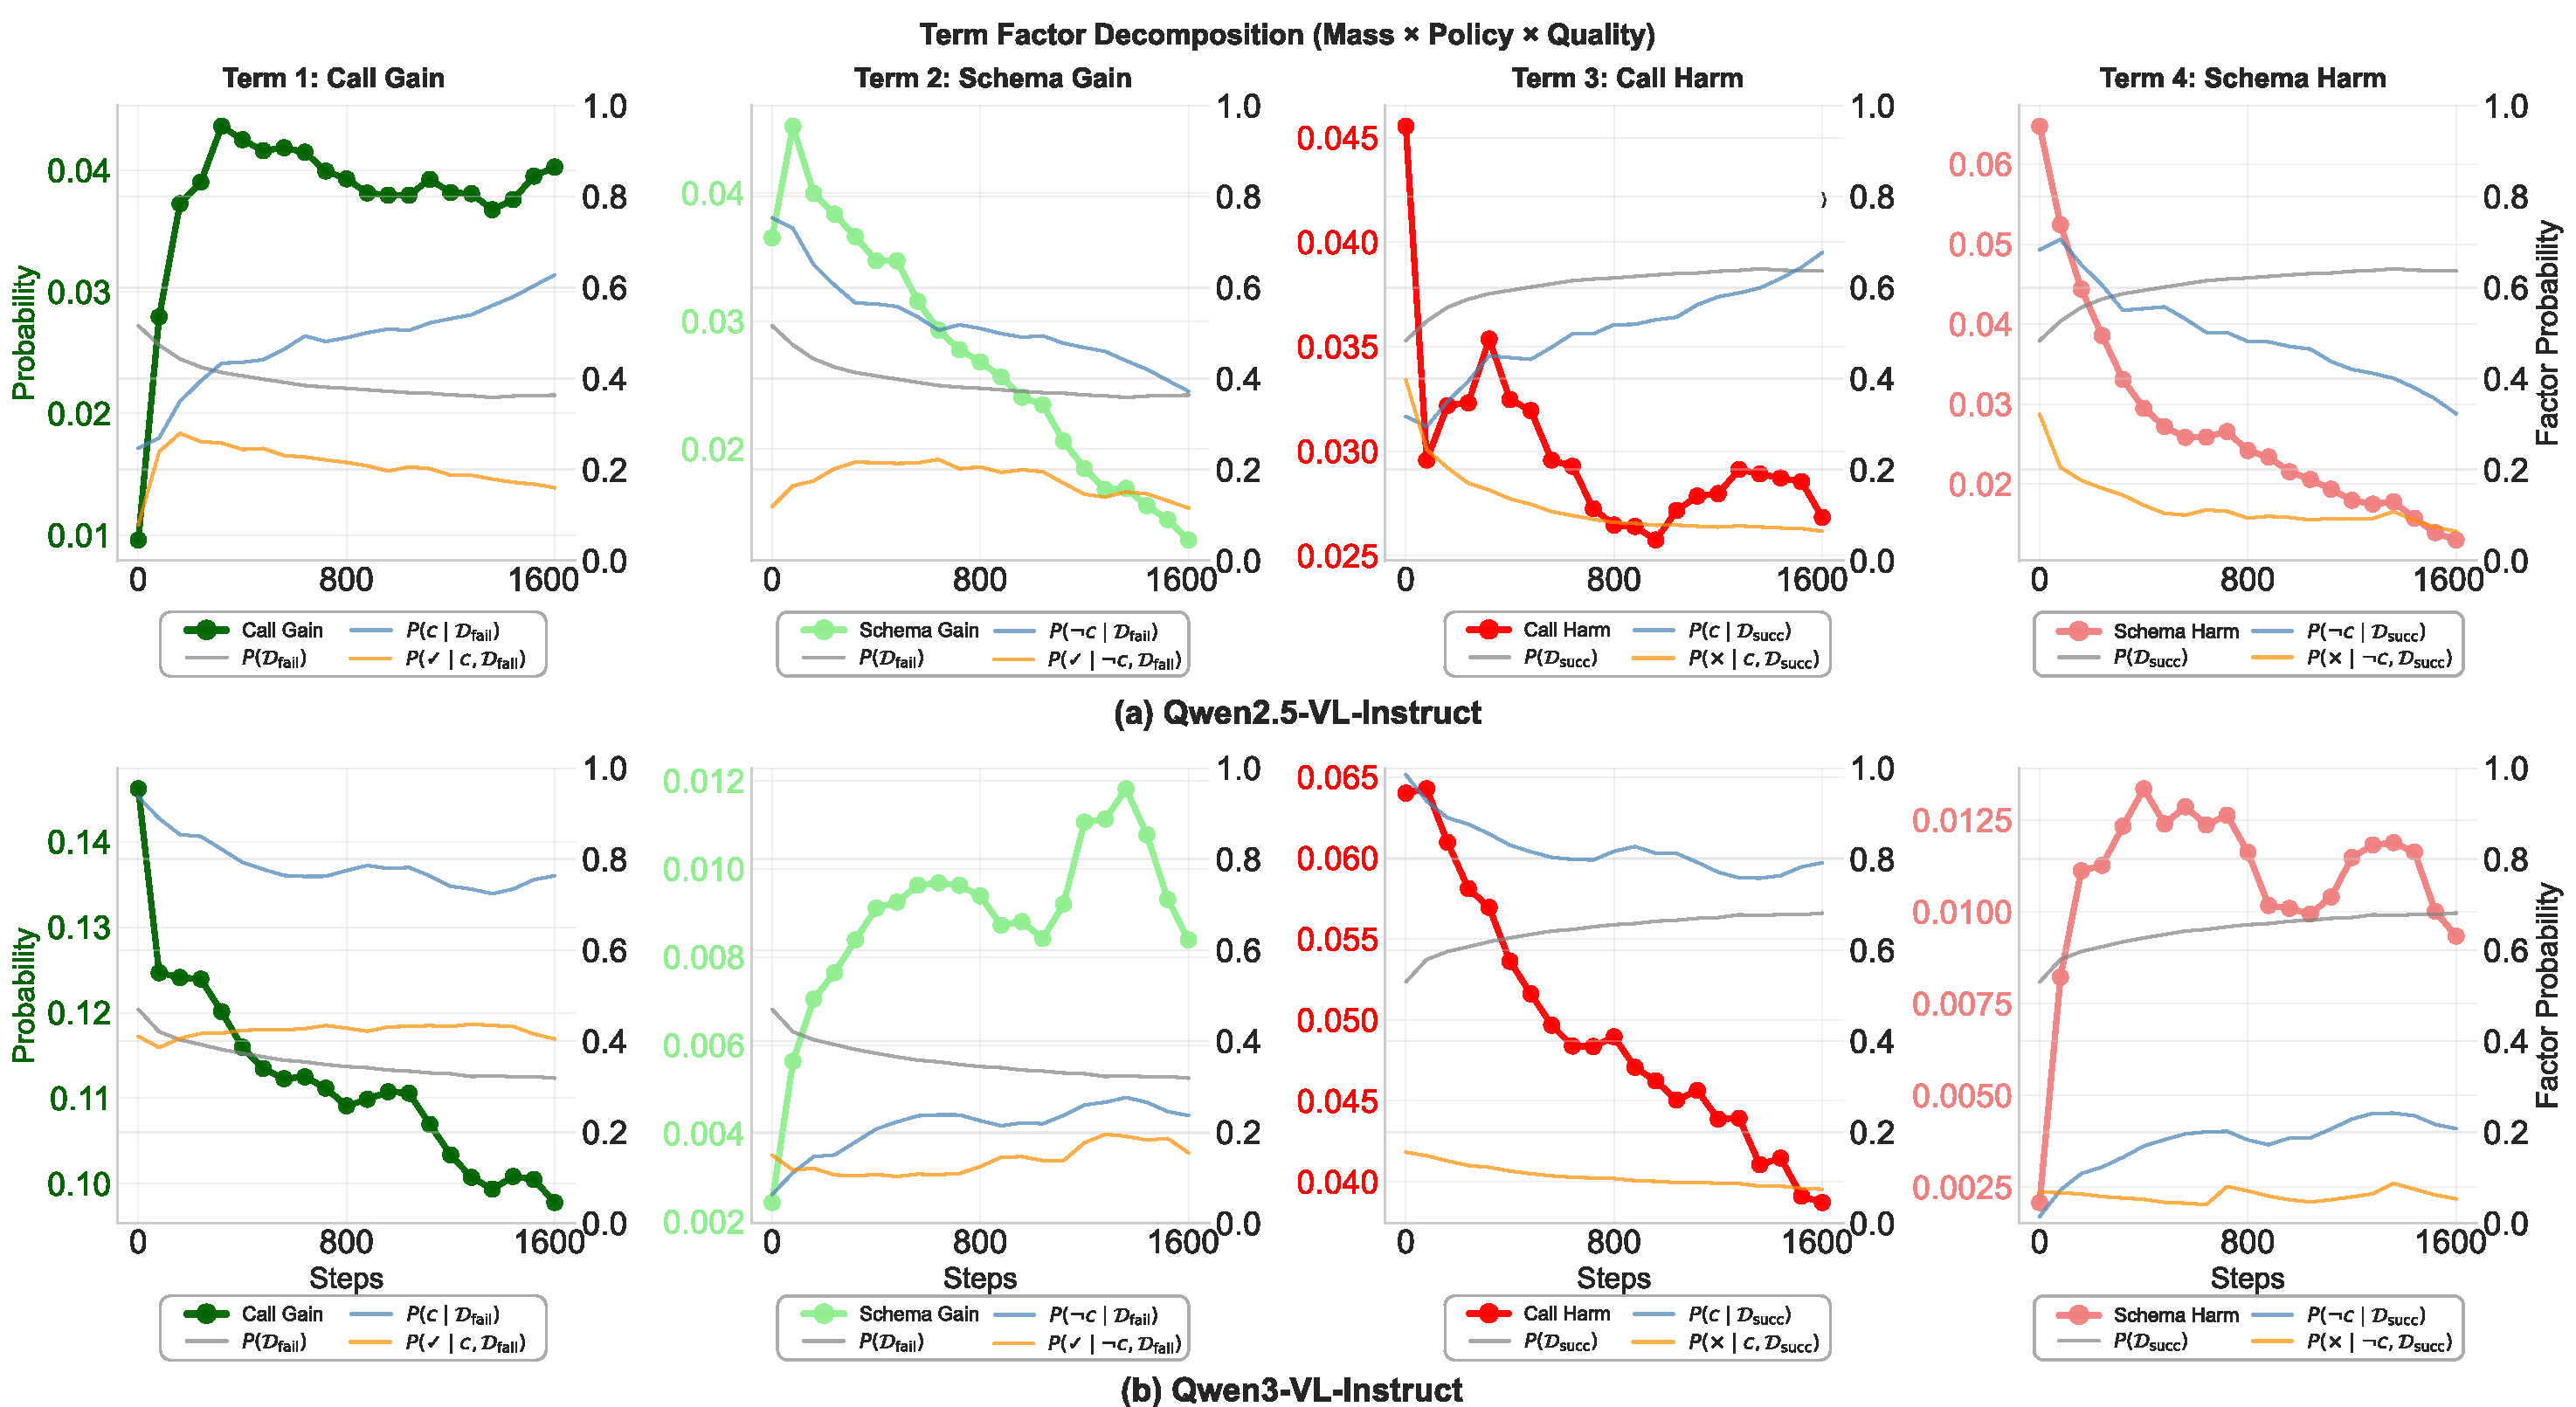
\includegraphics[width=0.98\linewidth]{figures/paper3/exp3_factor_decomposition.pdf}};
    \begin{scope}[x={(expthree.south east)},y={(expthree.north west)}]
      \filldraw[
        fill=white,
        fill opacity=0.95,
        draw=none
      ] (0.000,0.02) rectangle (0.255,0.935);
      \filldraw[
        fill=white,
        fill opacity=0.95,
        draw=none
      ] (0.495,0.02) rectangle (0.74,0.935);
      \node[
        text width=0.235\linewidth,
        align=left,
        inner sep=0pt
      ] at (0.125,0.72) {%
        {\fontsize{6.2}{7.3}\selectfont
        \textcolor{green!40!black}{\textbf{Qwen2.5-VL: Schema Gain} $\downarrow$}\\[-0.05em]
        \textcolor{red!75!black}{\textbf{Qwen2.5-VL: Schema Harm} $\downarrow$}\\[0.25em]
        RL reduces sensitivity to the tool schema.}
      };
      \node[
        text width=0.235\linewidth,
        align=left,
        inner sep=0pt
      ] at (0.618,0.28) {%
        {\fontsize{6.2}{7.3}\selectfont
        \textcolor{green!40!black}{\textbf{Qwen3-VL: Schema Gain/Harm}}\\[-0.05em]
        remain marginal $(<0.01)$\\[0.25em]
        Prior Crop-and-Zoom familiarity reduces schema effects.}
      };
    \end{scope}
  \end{tikzpicture}

  \vspace{-0.08cm}
  \begin{flushright}
    {\fontsize{5.5}{5}\selectfont \textcolor{darkgray}{[2025.10-2026.01]~~\textit{What Does Vision Tool-Use Reinforcement Learning Really Learn? Disentangling Tool-Induced and Intrinsic Effects for Crop-and-Zoom}, Ma et al.}}
  \end{flushright}
\end{frame}

\molochset{progressbar=foot}

\begin{frame}{\Large What Should Future Tool-Use RL Learn?}
  \begin{columns}[T,onlytextwidth]
    \begin{column}{0.65\textwidth}
      \centering
      \vspace{1.45cm}
      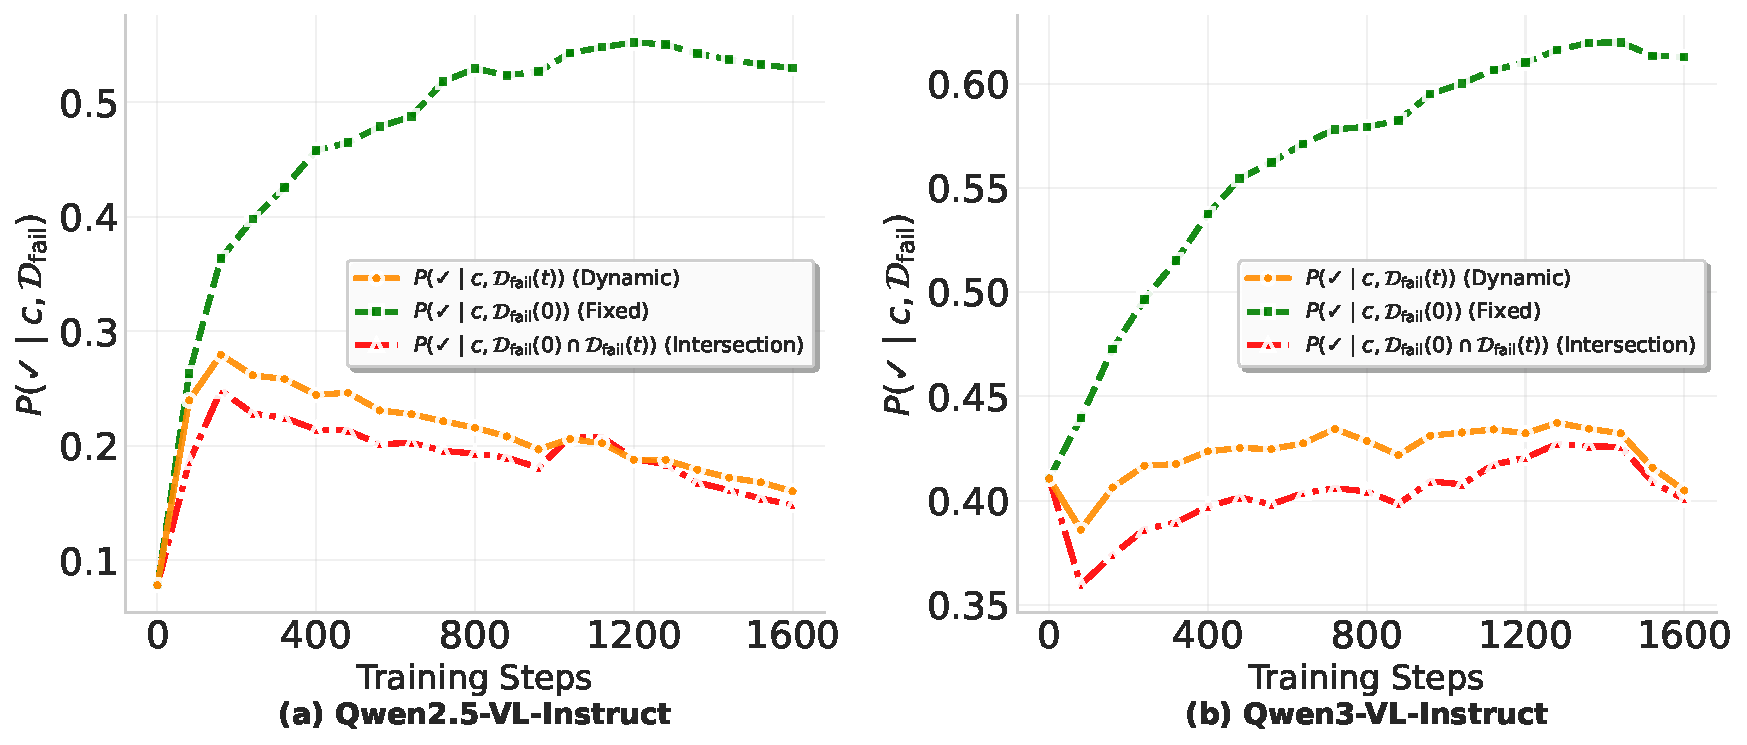
\includegraphics[width=0.98\linewidth]{figures/paper3/exp4_moving_failure_set.pdf}
    \end{column}
    \begin{column}{0.34\textwidth}
      \vspace{1.45cm}
      {\fontsize{8}{10.2}\selectfont
      \textbf{Tool-use goal: expand the model boundary}
      \[
        x \in \mathcal D_{\mathrm{fail}}(t):
        \quad
        \times_{\mathrm{w/o\ tool}}
        \xrightarrow{\;c\;}
        \checkmark_{\mathrm{w/\ tool}}
      \]

      \vspace{-0.35cm}
      \textbf{Current RL mainly learns:}
      \[
        P(\times \mid c,\mathcal D_{\mathrm{succ}}(t)) \downarrow
      \]

      \vspace{-0.35cm}
      \textbf{Missing target:}
      \[
        P(\checkmark \mid c,\mathcal D_{\mathrm{fail}}(t)) \uparrow
      \]
      }
    \end{column}
  \end{columns}

  \begin{flushright}
    \vspace{1.62cm}
    {\fontsize{5.5}{5}\selectfont \textcolor{darkgray}{[2025.10-2026.01]~~\textit{What Does Vision Tool-Use Reinforcement Learning Really Learn? Disentangling Tool-Induced and Intrinsic Effects for Crop-and-Zoom}, Ma et al.}}
  \end{flushright}
\end{frame}

\molochset{progressbar=foot}
